% Options for packages loaded elsewhere
\PassOptionsToPackage{unicode}{hyperref}
\PassOptionsToPackage{hyphens}{url}
%
\documentclass[
  9pt,
  english,
  ,jou,floatsintext]{apa6}
\usepackage{amsmath,amssymb}
\usepackage{lmodern}
\usepackage{ifxetex,ifluatex}
\ifnum 0\ifxetex 1\fi\ifluatex 1\fi=0 % if pdftex
  \usepackage[T1]{fontenc}
  \usepackage[utf8]{inputenc}
  \usepackage{textcomp} % provide euro and other symbols
\else % if luatex or xetex
  \usepackage{unicode-math}
  \defaultfontfeatures{Scale=MatchLowercase}
  \defaultfontfeatures[\rmfamily]{Ligatures=TeX,Scale=1}
\fi
% Use upquote if available, for straight quotes in verbatim environments
\IfFileExists{upquote.sty}{\usepackage{upquote}}{}
\IfFileExists{microtype.sty}{% use microtype if available
  \usepackage[]{microtype}
  \UseMicrotypeSet[protrusion]{basicmath} % disable protrusion for tt fonts
}{}
\makeatletter
\@ifundefined{KOMAClassName}{% if non-KOMA class
  \IfFileExists{parskip.sty}{%
    \usepackage{parskip}
  }{% else
    \setlength{\parindent}{0pt}
    \setlength{\parskip}{6pt plus 2pt minus 1pt}}
}{% if KOMA class
  \KOMAoptions{parskip=half}}
\makeatother
\usepackage{xcolor}
\IfFileExists{xurl.sty}{\usepackage{xurl}}{} % add URL line breaks if available
\IfFileExists{bookmark.sty}{\usepackage{bookmark}}{\usepackage{hyperref}}
\hypersetup{
  pdftitle={Examining side effect variability of antipsychotic treatment in schizophrenia spectrum disorders: A meta-analysis of variance},
  pdfauthor={Maria S. Neumeier1, Stephanie Homan, Ph.D.1, Stefan Vetter, M.D.1, Erich Seifritz, M.D.1, John M. Kane, M.D.2,3,4, Maximilian Huhn, M.D.5, Stefan Leucht, M.D.5, \& Philipp Homan, M.D., Ph.D.1,2,3,4*},
  pdflang={en-EN},
  hidelinks,
  pdfcreator={LaTeX via pandoc}}
\urlstyle{same} % disable monospaced font for URLs
\usepackage{longtable,booktabs,array}
\usepackage{calc} % for calculating minipage widths
% Correct order of tables after \paragraph or \subparagraph
\usepackage{etoolbox}
\makeatletter
\patchcmd\longtable{\par}{\if@noskipsec\mbox{}\fi\par}{}{}
\makeatother
% Allow footnotes in longtable head/foot
\IfFileExists{footnotehyper.sty}{\usepackage{footnotehyper}}{\usepackage{footnote}}
\makesavenoteenv{longtable}
\usepackage{graphicx}
\makeatletter
\def\maxwidth{\ifdim\Gin@nat@width>\linewidth\linewidth\else\Gin@nat@width\fi}
\def\maxheight{\ifdim\Gin@nat@height>\textheight\textheight\else\Gin@nat@height\fi}
\makeatother
% Scale images if necessary, so that they will not overflow the page
% margins by default, and it is still possible to overwrite the defaults
% using explicit options in \includegraphics[width, height, ...]{}
\setkeys{Gin}{width=\maxwidth,height=\maxheight,keepaspectratio}
% Set default figure placement to htbp
\makeatletter
\def\fps@figure{htbp}
\makeatother
\setlength{\emergencystretch}{3em} % prevent overfull lines
\providecommand{\tightlist}{%
  \setlength{\itemsep}{0pt}\setlength{\parskip}{0pt}}
\setcounter{secnumdepth}{-\maxdimen} % remove section numbering
% Make \paragraph and \subparagraph free-standing
\ifx\paragraph\undefined\else
  \let\oldparagraph\paragraph
  \renewcommand{\paragraph}[1]{\oldparagraph{#1}\mbox{}}
\fi
\ifx\subparagraph\undefined\else
  \let\oldsubparagraph\subparagraph
  \renewcommand{\subparagraph}[1]{\oldsubparagraph{#1}\mbox{}}
\fi
% Manuscript styling
\usepackage{upgreek}
\captionsetup{font=singlespacing,justification=justified}

% Table formatting
\usepackage{longtable}
\usepackage{lscape}
% \usepackage[counterclockwise]{rotating}   % Landscape page setup for large tables
\usepackage{multirow}		% Table styling
\usepackage{tabularx}		% Control Column width
\usepackage[flushleft]{threeparttable}	% Allows for three part tables with a specified notes section
\usepackage{threeparttablex}            % Lets threeparttable work with longtable

% Create new environments so endfloat can handle them
% \newenvironment{ltable}
%   {\begin{landscape}\begin{center}\begin{threeparttable}}
%   {\end{threeparttable}\end{center}\end{landscape}}
\newenvironment{lltable}{\begin{landscape}\begin{center}\begin{ThreePartTable}}{\end{ThreePartTable}\end{center}\end{landscape}}

% Enables adjusting longtable caption width to table width
% Solution found at http://golatex.de/longtable-mit-caption-so-breit-wie-die-tabelle-t15767.html
\makeatletter
\newcommand\LastLTentrywidth{1em}
\newlength\longtablewidth
\setlength{\longtablewidth}{1in}
\newcommand{\getlongtablewidth}{\begingroup \ifcsname LT@\roman{LT@tables}\endcsname \global\longtablewidth=0pt \renewcommand{\LT@entry}[2]{\global\advance\longtablewidth by ##2\relax\gdef\LastLTentrywidth{##2}}\@nameuse{LT@\roman{LT@tables}} \fi \endgroup}

% \setlength{\parindent}{0.5in}
\setlength{\parskip}{0pt plus 0pt minus 0pt}
% \setlength{\parskip}{0pt}

% \usepackage{etoolbox}
\makeatletter
\patchcmd{\HyOrg@maketitle}
  {\section{\normalfont\normalsize\abstractname}}
  {\section*{\normalfont\normalsize\abstractname}}
  {}{\typeout{Failed to patch abstract.}}
\patchcmd{\HyOrg@maketitle}
  {\section{\protect\normalfont{\@title}}}
  {\section*{\protect\normalfont{\@title}}}
  {}{\typeout{Failed to patch title.}}
\makeatother
\shorttitle{Variability of side effects}
\leftheader{}
\usepackage{dblfloatfix}


\usepackage{csquotes}
\usepackage{libertine}
\captionsetup[figure]{font=footnotesize,labelfont=bf}
\newcommand{\beginsupplement}{\setcounter{table}{0}
\renewcommand{\thetable}{S\arabic{table}}
\setcounter{figure}{0}
\renewcommand{\thefigure}{S\arabic{figure}}}
\ifxetex
  % Load polyglossia as late as possible: uses bidi with RTL langages (e.g. Hebrew, Arabic)
  \usepackage{polyglossia}
  \setmainlanguage[]{english}
\else
  \usepackage[main=english]{babel}
% get rid of language-specific shorthands (see #6817):
\let\LanguageShortHands\languageshorthands
\def\languageshorthands#1{}
\fi
\ifluatex
  \usepackage{selnolig}  % disable illegal ligatures
\fi
\newlength{\cslhangindent}
\setlength{\cslhangindent}{1.5em}
\newlength{\csllabelwidth}
\setlength{\csllabelwidth}{3em}
\newenvironment{CSLReferences}[2] % #1 hanging-ident, #2 entry spacing
 {% don't indent paragraphs
  \setlength{\parindent}{0pt}
  % turn on hanging indent if param 1 is 1
  \ifodd #1 \everypar{\setlength{\hangindent}{\cslhangindent}}\ignorespaces\fi
  % set entry spacing
  \ifnum #2 > 0
  \setlength{\parskip}{#2\baselineskip}
  \fi
 }%
 {}
\usepackage{calc}
\newcommand{\CSLBlock}[1]{#1\hfill\break}
\newcommand{\CSLLeftMargin}[1]{\parbox[t]{\csllabelwidth}{#1}}
\newcommand{\CSLRightInline}[1]{\parbox[t]{\linewidth - \csllabelwidth}{#1}\break}
\newcommand{\CSLIndent}[1]{\hspace{\cslhangindent}#1}

\title{Examining side effect variability of antipsychotic treatment in schizophrenia spectrum disorders: A meta-analysis of variance}
\author{Maria S. Neumeier\textsuperscript{1}, Stephanie Homan, Ph.D.\textsuperscript{1}, Stefan Vetter, M.D.\textsuperscript{1}, Erich Seifritz, M.D.\textsuperscript{1}, John M. Kane, M.D.\textsuperscript{2,3,4}, Maximilian Huhn, M.D.\textsuperscript{5}, Stefan Leucht, M.D.\textsuperscript{5}, \& Philipp Homan, M.D., Ph.D.\textsuperscript{1,2,3,4*}}
\date{}


\affiliation{\vspace{0.5cm}\textsuperscript{1} University Hospital of Psychiatry Zurich, Zurich, Switzerland.\\\textsuperscript{2} Center for Psychiatric Neuroscience, Feinstein Institute for Medical Research, Manhasset, NY, USA.\\\textsuperscript{3} Division of Psychiatry Research, Zucker Hillside Hospital, Northwell Health, New York, NY, USA.\\\textsuperscript{4} Department of Psychiatry, Zucker School of Medicine at Northwell/Hofstra, Hempstead, NY, USA.\\\textsuperscript{5} Department of Psychiatry and Psychotherapy, Technical University of Munich, School of Medicine, Munich, Germany.}

\abstract{
Side effects of antipsychotic
drugs play a key role in non-adherence of treatment in schizophrenia
spectrum disorders (SSD). While clinical observations suggest
that side effect variability between patients may be considerable,
statistical evidence is
required to confirm this. Here, we hypothesized to find larger side effect
variability under treatment compared with control. We included double-blind,
placebo-controlled, randomized controlled trials (RCTs) of adults with
a diagnosis of SSD treated with 1 out of 14 antipsychotics.
Standard deviations of the pre-post treatment differences of weight
gain, prolactin levels, and corrected QT (QTc) times were extracted.
The outcome measure was the variability ratio of treatment to control for
individual antipsychotic drugs and the overall variability ratio of
treatment to control across RCTs. Individual variability ratios were
weighted by the inverse-variance method and entered into a
random-effects model. We included N = 16578 patients for weight
gain, N = 16633 patients for prolactin levels, and N = 10384
patients for QTc time. Variability ratios (VR) were significantly
increased for weight gain (VR = 1.08; 95\% CI: 1.02 - 1.14; P = 0.004) and
prolactin levels (VR = 1.38; 95\% CI: 1.17 - 1.62; P \textless{} 0.001) but did not
reach significance for QTc time (VR = 1.05; 95\% CI: 0.98 - 1.12; P = 0.135).
We found marked differences between individual antipsychotics and
increased variability in side effects in patients under treatment
with antipsychotics suggesting that subgroups of patients or
individual patients may benefit from treatment allocation through
stratified or personalized medicine.
}



\begin{document}
\maketitle

\hypertarget{introduction}{%
\section{Introduction}\label{introduction}}

Antipsychotics are a fundamental component in the treatment of
schizophrenia spectrum disorders (SSD). Yet, a major problem are side
effects which play a key role in non-adherence and
discontinuation.\textsuperscript{1--5} A common hypothesis among researchers and clinicians alike
is that although side effects are pervasive, not all patients are equally
susceptible, even when they are treated with the same drug.\textsuperscript{6}
However, empirical support for this hypothesis is lacking, as randomized
controlled trials (RCTs) or conventional meta-analyses by design cannot
answer whether such side effect variability does exist.\textsuperscript{7,8}

While it is well-established that antipsychotics are associated
with sides effects for the average patient, the approach we are taking
with this study moves beyond comparing group averages but instead
compares group variances. By comparing variances our study can
for the first time test the hypothesis that there is indeed reason
to believe that subgroups or even individual patients differ in
their susceptibility to side effects -- something that an analysis
focused on group averages cannot do.

To date, studies have established the efficacy, safety, and side effect
profiles of antipsychotic medications by averaging these indices across
groups of patients. Such studies can provide us with average side effects
for specific drugs, but they cannot tell us anything about individual
patients or subgroups.\textsuperscript{9,10} Nevertheless, before searching
for potential biomarkers that might predict individual susceptibility, we
should first quantify the extent to which such predictors are truly needed.

An approach to answering this question is to shift the focus from the
means to the variances of side effects.\textsuperscript{11} By comparing the
variances between treatment and control groups of RCTs,\textsuperscript{12}
greater variability in treatment would mean that some patients are more
susceptible to side effects than others.\textsuperscript{11} Note that this
method\textsuperscript{13} has recently been applied for
antipsychotics,\textsuperscript{7} antidepressants,\textsuperscript{8,14,15} and brain stimulation,\textsuperscript{16} but in
the context of treatment effect variability. It is worth noting that these
studies found little evidence for treatment effect
variability.\textsuperscript{7,8,14,15}
Importantly, in the case of pre-post differences used as input for a
meta-analysis of variance it is crucial to think carefully about the way
the variability ratio is expressed,\textsuperscript{12,15,17} as the use of the coefficient of variation ratio (CVR)
that has been proposed as an alternative of the variability ratio
(VR)\textsuperscript{12} may lead to unreliable results.\textsuperscript{13,17}

A recently published study investigated the individual treatment
response in antipsychotics and brought surprising
results.\textsuperscript{7,18} By comparing the
variability between treatment and control groups, no evidence was found
for an increase in variability in the treatment group. What might sound
counter-intuitive at first raises the question of how big the need for
precision medicine really is. However, that study evaluated the evidence
for treatment effect variability. It is possible that although such
variability in treatment effects is not as high as sometimes assumed,\textsuperscript{19} it does exist in the susceptibility for side effects. In
other words, even if there is little variability in response to treatment
between patients, there may still be enough variability in side effects to
justify a need for precision medicine. If true, then this would support
optimization of treatment allocation with respect to side effect
profiles.\textsuperscript{20}

Side effects that are particularly relevant to antipsychotic treatment
include weight gain,\textsuperscript{5} hyperprolactinemia, and QTc
prolongation.\textsuperscript{20} Weight gain is a frequently observed side
effect that can negatively impact one's physical health and thus may
also influence treatment adherence. Every additional kilogram of weight
gain can contribute to an increased risk of heart
failure,\textsuperscript{21} cardiovascular disease,\textsuperscript{22} and
diabetes.\textsuperscript{23} In addition, treatment discontinuation is often
seen in patients with increase of weight under treatment.\textsuperscript{24}
High prolactin levels can lead to symptoms like decreased bone mass,
gallactorhea, and fertility problems in men and women. Further possible
symptoms include menstrual disturbances in female patients and decreased
libido and erectile dysfunction in male patients.\textsuperscript{25} These
symptoms are frequent, but often underreported by patients and unnoticed
as well as untreated by clinicians.\textsuperscript{26,27} They
furthermore might lead to loss in quality of life and might be a reason
for treatment discontinuation\textsuperscript{1,28} and subsequent
illness relapse, which together with persistent positive symptoms\textsuperscript{29--32} may severely
impact recovery and therapeutic alliance.\textsuperscript{33} Prolongation of
QTc was observed in 7 of 14 antipsychotics compared by placebo in the
inter-group comparison by Huhn and colleagues.\textsuperscript{6} Importantly,
\emph{torsade de pointes} tachycardia and sudden cardiac death are possible
severe consequences of QTc prolongation.\textsuperscript{34} Such cardiac events
are one of the factors that lead to the loss of life expectancy observed
in patients with SSD.\textsuperscript{35--37}

In summary, antipsychotic side effects are highly relevant for
long-term outcome and adherence in treatment of positive symptoms in
SSD. The question remains whether variability in side effects is high
enough to warrant efforts of treatment stratification or
personalisation. If there is little or no evidence for variability in
side effects there might not be a need for stratification or personalization
and the already widely available data provided by
intergroup comparisons might offer reasonable estimates for the
individual patient. Thus, we compared the variances of side effects
including weight gain, prolactin level and QTc-time between treatment
and control groups to address this question and to evaluate the
evidence for the presence of side effect variability. Based on the
clinical impression that patients seem to vary in their susceptibility
to side effects, we hypothesized that the variability in side effects
would be higher in the treatment compared with the control groups
across all published trials of antipsychotics in SSD.\textsuperscript{6}

\hypertarget{methods}{%
\section{Methods}\label{methods}}

\hypertarget{search-strategy-and-selection-criteria}{%
\subsection{Search strategy and selection criteria}\label{search-strategy-and-selection-criteria}}

We used the data from the recent meta-analysis by Huhn and
colleagues.\textsuperscript{6} That study included placebo-controlled published
and unpublished trials investigating orally administered atypical
(second generation) antipsychotics and typical (first generation)
antipsychotics in adults with schizophrenia spectrum disorders; and
excluded patients with first episode psychosis, treatment resistance,
mainly negative symptoms, comorbidity with other mental or physical
illnesses and relapse-prevention studies. Long- and short-acting
intramuscular injections were also excluded (as they are often used in
relapse prevention or emergency treatment) and studies from mainland
China were excluded because of data quality concerns.\textsuperscript{38}
Data sources were MEDLINE, Cochrane Central Register of Controlled Trials
(CENTRAL), Embase, Biosis, PsycINFO, PubMed, ClinicalTrials.gov, WHO
International Clinical Trials Registry Platform and the US Food and Drug
Administration until January 8 2019. Data quality and validity were
ensured by following the PRISMA guidelines.\textsuperscript{39} For missing
data, we also contacted study authors.

We decided to investigate weight gain, prolactin elevation and
QTc prolongation because these side effects are particularly relevant,\textsuperscript{5,20} and quantifiable metric data were
available in most studies. Other side effects such as
extrapyramidal motor symptoms (EPS), sedation and diabetes can be
equally burdensome and certainly pose a health risk to patients.
However, those have often not been quantified in studies but rather
assessed qualitatively (e.g.~through categorical variables such as
EPS: yes/no; sedation: yes/no; diabetes: treated/untreated).
These types of variables did not allow us to estimate variability
and so we had to restrain from including them in the analysis.

For the analysis, we used the standard deviations of pre-post
differences in side effects. The primary outcome was the
overall variability ratio of side effects in treatment versus control groups.
Standard deviations (SD) and number of patients (N) were
extracted for weight gain, prolactin level and QTc time. The units used
were kg for weight gain, ng/mL for prolactin levels, and ms for QTc
time. Some studies provided data for all of the three side effects,
whereas the majority of the studies contained less data (see Results).

\hypertarget{statistical-analysis}{%
\subsection{Statistical analysis}\label{statistical-analysis}}

If patients or subgroups differ in their susceptibility to side effects,
we would expect to observe increased variances in the treatment
compared with the control group. To test this, we computed the log
variability ratio (log VR) by comparing the relative variability of
side effects under treatment versus control:

\[\textrm{log VR}=\textrm{log}\left(\frac{\textrm{SD}_{\textrm{Tx}}}{\textrm{SD}_{\textrm{Ct}}} \right) +
\frac{1}{2(n_{\textrm{Tx}}-1)} - \frac{1}{2(n_{\textrm{Ct}}-1)} \],

where \(\textrm{SD}_{\textrm{Tx}}\) was the reported sample SD for side
effects under treatment, \(\textrm{SD}_{\textrm{Ct}}\) was the reported
sample SD for side effects under control, \(n_{\textrm{Tx}}\) was the
treatment sample size, and \(n_{\textrm{Ct}}\) the control sample size. The
corresponding sampling variance (\(s_{\textrm{log VR}}^2\)) for each
comparison can be expressed as follows:

\[ s_{\textrm{log VR}}^2 = \frac{1}{2(n_{\textrm{Tx}}-1)} + \frac{1}{2(n_{\textrm{Ct}}-1)}\].

The individual variability ratios were weighted with the inverse of
this sampling variance\textsuperscript{40} and entered into a
random-effects model to quantify the overall variability ratio of side
effects. For better interpretability, results were back-transformed from
the logarithmic scale. Here, a variability ratio greater than one would
indicate a higher side effect variability in treatment compared with
control, whereas a variability ratio smaller than one would indicate less
side effect variability under treatment compared with control.

\hypertarget{data-and-code-availability}{%
\subsection{Data and code availability}\label{data-and-code-availability}}

The analysis was performed from September 2019 to May 2020, using the
R package metafor\textsuperscript{40}(version 2.4.0).
The manuscript was produced with the R packages rmarkdown
(version 2.6); represearch
(version 0.0.0.9000;
\url{https://github.com/phoman/represearch/});
knitr (version 1.30); and
papaja (version 0.1.0.9997).
All data and code are freely available online to ensure reproducibility at
\url{https://github.com/homanlab/sideeffects/}.

\hypertarget{results}{%
\section{Results}\label{results}}

\hypertarget{overall-reporting-details}{%
\subsection{Overall reporting details}\label{overall-reporting-details}}

Together, we screened N = 151 studies with 14 different
antipsychotics from the original meta-analysis by Huhn and
colleagues\textsuperscript{6} as these studies reported data on at least
one of the three side effects that we were interested in. Of these studies,
N = 94
(62\%)
had missing variance measures despite reported means for at least
one of the three side effects. We thus included the N = 60
(40\%) studies that did
report variance measures for at least one of the side effects of interest.

\hypertarget{weight-gain}{%
\subsection{Weight gain}\label{weight-gain}}

For weight gain, we included 51 RCTs, yielding 72
comparisons of antipsychotic drugs with placebo to investigate the individual
occurrence of weight gain in patients. All together we included
N = 16578 patients diagnosed with schizophrenia or schizoaffective
disorder. There were 11373 (69\%)
patients randomly allocated to the treatment group, and
5205 (31\%) to the placebo
group. Patients in the treatment group received 1 out of 14
investigated antipsychotic drugs. Individual comparisons between
drugs across studies indicated marked differences between individual
antipsychotics. The VR for chlorpromazine, cariprazine, and sertindole was
smaller than 1. The VR for ziprasidone, iloperidone, and brexpiprazole
was 1. The VR for asenapine, risperidone, olanzapine, lurasidone,
aripiprazol, paliperidone, haloperidol, and quetiapine was greater than 1
(VR = 1.08; 95\% CI: 1.02 - 1.14; P = 0.004; Figure \ref{fig:fig2}). Overall, the
variability for weight gain was higher under treatment than
under control (VR = 1.08; 95\% CI: 1.02 - 1.14; P = 0.004; Figure \ref{fig:fig1}).

\begin{figure}
\centering
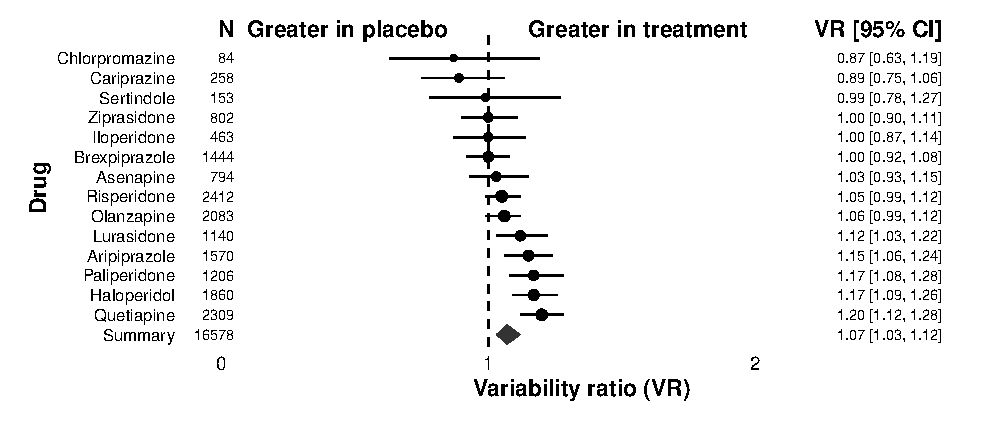
\includegraphics{../output/figures/weightsd_fig2.pdf}
\caption{\label{fig:fig2}Variability ratio for weight gain for individual
antipsychotics. The forest plot shows the VR together with its 95\%
confidence interval (CI) for treatment versus placebo. All included studies\textsuperscript{41--95}
are also listed in Table S1.}
\end{figure}

\hypertarget{hyperprolactinemia}{%
\subsection{Hyperprolactinemia}\label{hyperprolactinemia}}

For hyperprolactinemia, we included 50 RCTs, with 71
comparisons of antipsychotic drugs with placebo. All together we
included N = 16633 patients diagnosed with schizophrenia or
schizoaffective disorder. There were 11409
(69\%) patients randomly allocated to
the treatment group, and 5224
(31\%) to the placebo group. Patients
in the treatment group received 1 out of 13 investigated antipsychotic
drugs. Individual comparisons between drugs across studies indicated
marked differences between individual antipsychotics. The VR for
iloperidone and brexpiprazole was smaller than 1. The VR for aripiprazole,
asenapine, risperidone, cariprazine, sertindole, quetiapine, ziprasidone,
lurasidone, haloperidol, olanzapine, and paliperidone was greater than 1
(VR = 1.38; 95\% CI: 1.17 - 1.62; P \textless{} 0.001; Figure \ref{fig:fig4}).
Overall, the variability for hyperprolactinemia was higher under treatment
than under control (VR = 1.38; 95\% CI: 1.17 - 1.62; P \textless{} 0.001; Figure \ref{fig:fig3}).

\begin{figure}
\centering
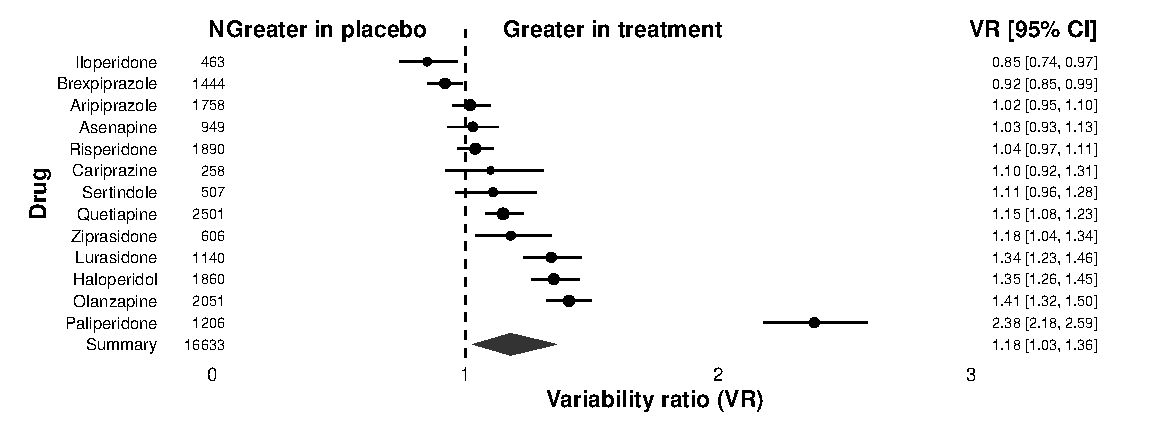
\includegraphics{../output/figures/prolactinsd_fig2.pdf}
\caption{\label{fig:fig4}Variability ratio for hyperprolactinemia for individual
antipsychotics. The forest plot shows the VR together with its 95\%
confidence interval (CI) for treatment versus placebo. All included studies\textsuperscript{41,42,44--48,50--58,60,62,64,65,67--69,72,74--79,82--92,94--100}
are also listed in Table S1.}
\end{figure}

\hypertarget{qtc-prolongation}{%
\subsection{QTc prolongation}\label{qtc-prolongation}}

For QTc prolongation, we included 29 RCTs, with 46
comparisons of antipsychotic drugs with placebo. All together we
included N = 10384 patients diagnosed with schizophrenia or
schizoaffective disorder. There were 7439
(72\%) patients randomly allocated to
the treatment group, and 2945
(28.00\%) to the placebo group. Patients
in the treatment group received 1 out of 11 investigated antipsychotic
drugs. Individual comparisons between drugs across studies indicated
marked differences between individual antipsychotics
(VR = 1.05; 95\% CI: 0.98 - 1.12; P = 0.135; Figure \ref{fig:fig6}).
The VR for ziprasidone, brexpiprazole, paliperidone, and olanzapine was
smaller than 1. The VR for iloperidone was 1. The VR for risperidone,
quetiapine, lurasidone, haloperidol, and sertindole was greater than 1.
Even though the variability for QTc prolongation was higher under
treatment than under control, the difference did not reach statistical
significance (VR = 1.05; 95\% CI: 0.98 - 1.12; P = 0.135; Figure \ref{fig:fig5}).

\begin{figure}
\centering
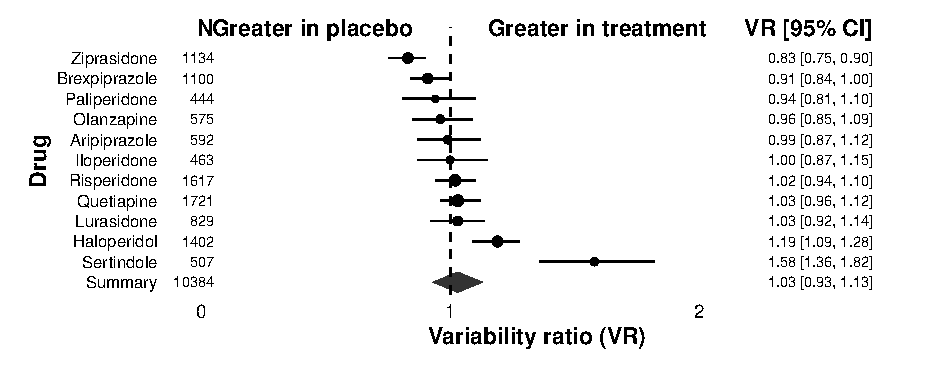
\includegraphics{../output/figures/qtcsd_fig2.pdf}
\caption{\label{fig:fig6}Variability ratio for QTC prolongation for individual
antipsychotics. The forest plot shows the VR together with its 95\%
confidence interval (CI) for treatment versus placebo. All included studies\textsuperscript{42,45,51,52,54--60,62,68,70,74,76--80,85,86,88,91,95,96,100}
are also listed in Table S1.}
\end{figure}

\hypertarget{discussion}{%
\section{Discussion}\label{discussion}}

\hypertarget{summary}{%
\subsection{Summary}\label{summary}}

This study assessed the variability in the three major side effects of
antipsychotic treatment in schizophrenia spectrum disorders. We
focused on side effects because their occurrence has a great impact on
treatment adherence and physical health of patients, and clinical
experience suggests a potential to improve treatment allocation by
taking into account the variability in side effect occurrence. We also
know from clinical trials and meta-analyses that some antipsychotics
are more associated with specific side effects than others. For
example, clozapine and olanzapine are strongly associated with weight
gain,\textsuperscript{6,20,101} QTc-time prolongation is
most distinct in sertindole and amisulpride,\textsuperscript{6} and prolactin
level elevation in paliperidone and risperidone.\textsuperscript{6} However,
these data cannot address the question whether there is variability in
subgroups or individual patients. Such side effect-by-subgroup or side
effect-by-patient interaction would be a prime example for the need of
a more stratified or personalized medicine, respectively, which
allocates treatments according to side effect profiles of subgroups or
individual patients. Overall, we found that the variability for weight
gain and prolactin elevation was indeed significantly increased in
patients who received treatment compared with those who received
placebo. For QTc prolongation, the increase was not
significant. Together, our results suggest that there is indeed marked
variability in the occurrence of side effects in antipsychotic
treatment. Variability also differed markedly between individual drugs.

\hypertarget{reporting}{%
\subsection{Reporting}\label{reporting}}

Altogether we included 43595 patients from 60
studies. The included studies provided data for treatment with 14
antipsychotic drugs for weight gain, 13 antipsychotic drugs
for hyperprolactinemia, and 11 antipsychotic drugs for
QTc prolongation compared to placebo. Only for about 40\% of studies
included in a previous meta-analysis\textsuperscript{6} variance data for at
least one of the side effects of interest (weight gain, prolactin
levels, QTc prolongation) were available. In about 62\% of the studies
included\textsuperscript{6} incomplete data existed such that means were reported
without a measure of variance. Although we did contact authors for missing
data whenever possible, we received missing data only for three studies.
In summary, consistent reporting of antipsychotic side effects,
specifically with respect to variability measures, is currently missing
in the literature and should be improved in future studies.

\hypertarget{weight-gain-1}{%
\subsection{Weight gain}\label{weight-gain-1}}

Weight gain, especially for second generation
antipsychotics,\textsuperscript{102} is a severe side effect that can
contribute to metabolic dysregulation. Importantly, every kg of weight
gain leads to a linear increase in the risk of cardiovascular
diseases,\textsuperscript{22} heart failure,\textsuperscript{21} and
diabetes.\textsuperscript{23} Clozapine, olanzapine, zotepine, and sertindole
have the most severe impact in gaining weight. Some studies showed
that a lower BMI at baseline\textsuperscript{103} and sex\textsuperscript{104} can
lead to more weight gain, whereas other studies found that male sex
and higher BMI at baseline are related to a higher risk of metabolic
disturbances.\textsuperscript{20} Our findings provide evidence that some
patients are indeed more susceptible to antipsychotic weight gain than
others, and that this susceptibility varies also between
medications. For example, for quetiapine we found that patients
differed in their susceptibility for weight gain while we did not find
such evidence for olanzapine and brexpiprazole, suggesting a potential
for stratified or personalized medicine for quetiapine but not
olanzapine and brexpiprazole. As antipsychotics in the treatment for
schizophrenia and related diseases is often recommended to be taken as
a relapse prevention for a longer period,\textsuperscript{105,106}
patients are likely to gain more weight during their treatment over
months and years. Together, this suggests that there is a potential to
improve long-term health and adherence by identifying the subgroups or
individual patients that are particularly prone to weight
gain. Preliminary evidence suggests that a dysregulated striatal
reward circuit contributes to this weight gain
susceptibility.\textsuperscript{5,107}

\hypertarget{hyperprolactinemia-1}{%
\subsection{Hyperprolactinemia}\label{hyperprolactinemia-1}}

Prolactin level elevations occur in up to 70\% of patients\textsuperscript{108}
under the treatment with antipsychotics. By blocking dopamine D2
receptors on lacotroph cells a disinhibition of the synthesis and
secretion of prolactin is observed.\textsuperscript{109,110} This
can lead to both short- and long-term side effects with potentially
severe impact on patients' health. Typical short-term effects include
galactorrhea, gynecomastia, menstrual irregularities, and sexual
dysfunction; a typical long-term result is
osteoporosis,\textsuperscript{111,112} and a potentially increased
risk in developing breast cancer in association with
hyperprolactinemia.\textsuperscript{113,114} Our findings suggest
that these risks may be particularly relevant for some patients but
not others, and more relevant for some antipsychotic drugs than
others. For example, a previous study found that prolactin level
elevations are more pronounced and more frequent in women than in
men.\textsuperscript{115} In addition, some antipsychotics such as
amisulpride, risperidone, and paliperidone are linked to a greater
elevation of prolactin.\textsuperscript{6,115} The striking
difference between risperidone (for which we did not find evidence for
significant variability in prolactin elevation) and paliperidone (for
which we did find such evidence) is puzzling as paliperidone is an
active metabolite of risperidone, and previous literature suggests
that paliperidone and risperidone lead to similar elevations in serum
prolactin concentrations.\textsuperscript{116} A possible
explanation is that the level of prolactin can be highly variable
based on multiple biological and methodological factors such as
stress, diurnal variation and type of assay performed. However, future
studies should pay particular attention to differences in
susceptibility to prolactinemia between these two antipsychotics. In
summary, and in line with the weight gain findings, our findigns
suggest that there is a potential to improve long-term health and
antipsychotic adherence by identifying the subgroups or individual
patients that are particularly likely to develop prolactin elevations
under antipsychotic treatment.

\hypertarget{qtc-prolongation-1}{%
\subsection{QTc prolongation}\label{qtc-prolongation-1}}

Prolongation of QTc is another important antipsychotic side effect as
cardiovascular diseases remain the most common cause of natural
mortality in schizophrenia spectrum disorders.\textsuperscript{117} Users of
antipsychotic medication are reported to have higher rates of sudden
cardiac death than nonusers.\textsuperscript{118} Prolongation of QTc (longer
than 450 ms in men and longer than 470 ms in women, respectively, when
corrected with Bazetts Formula\textsuperscript{119}) can contribute to
this.\textsuperscript{34} A prolongation of QTc can lead to \emph{torsade de
pointes} and subsequently to sudden death.\textsuperscript{120,121} The molecular pathway of this side effect is not
completely understood.\textsuperscript{122} It is known, however, that some
medications such as sertindole, amisulprid, and ziprasidone lead to
more QTc prolongation than others.\textsuperscript{6} Here, we found increased
variability for some antipsychotics such as haloperidol in QTc
prolongation. However, altogether we did not find a statistically
significant increase in variability for QTc prolongation, potentially
because a smaller number of studies were available which decreased
statistical power.

\hypertarget{limitations-and-strengths}{%
\subsection{Limitations and strengths}\label{limitations-and-strengths}}

Our meta-analysis had some limitations. First, the occurrence of side
effects might be a dose-dependent effect which could reflect a
higher/different VR in some studies. Dose-dependent means and standard
deviations are often missing but would be necessary to investigate
dose-dependent effects. Second, for QTc, a reduced number of studies was
available, potentially reducing statistical power to detect a
significant variability increase. Third, our sample did not include
pre-defined subgroups including patients with first-episode psychosis
and treatment-resistant patients to create the most homogeneous sample
possible. Finally, our method cannot determine
whether the increased variability is due to variability differences in
subgroups or individual patients.\textsuperscript{11} The particular strength
of our study is that we included all available studies of antipsychotic
treatment in SSD reporting variability measures for side effects of
interest. To our knowledge, this is the first comprehensive study that
provides evidence for substantial variability in side effects.

\hypertarget{conclusion}{%
\subsection{Conclusion}\label{conclusion}}

While we did not find convincing evidence that patients differed in
their susceptibility to QTc prolongation, we did find such evidence
for weight gain and prolactin elevation: for half of all
antipsychotics (7 out of 14) we can assume that subgroups of patients
or even individual patients would benefit from specific treatment
allocation through stratified or personalized medicine,
respectively. Such efforts in precision medicine might be crucial to
improve adherence and long-term health under antipsychotic treatment.

\hypertarget{acknowledgements}{%
\section{Acknowledgements}\label{acknowledgements}}

The authors thank Majnu John, PhD, for advice on the analysis of the
current study and Ellen Ji, PhD, for her thoughtful comments on the
manuscript. These individuals received no additional compensation,
outside of their usual salary, for their contributions.

\hypertarget{fundingsupport}{%
\section{Funding/Support}\label{fundingsupport}}

PH is supported by a NARSAD grant from the Brain \& Behavior Research
Foundation (28445) and by a Research Grant from the Novartis Foundation
(20A058).

\hypertarget{conflict-of-interest}{%
\section{Conflict of interest}\label{conflict-of-interest}}

In the last 3 years Dr.~Leucht has received honoraria for service as a
consultant or adviser and/or for lectures from Angelini, Böhringer
Ingelheim, Geodon\&Richter, Janssen, Johnson\&Johnson, Lundbeck, LTS
Lohmann, MSD, Otsuka, Recordati, SanofiAventis, Sandoz, Sunovion,
TEVA. Dr.~Kane reported grants from Otsuka, Lundbeck and Janssen, as
well as other from Alkermes, Allergan, Forum, Genentech, Lundbeck,
Intracellular Therapies, Janssen, Johnson \& Johnson, Merck, Neurocrine,
Otsuka, Pierre Fabre, Reviva, Roche, Sunovion, Takeda, Teva, Vanguard
Research Group, and LB Pharmaceuticals outside of the submitted work. No
other disclosures were reported.

\hypertarget{author-contributions}{%
\section{Author contributions}\label{author-contributions}}

MSN co-analyzed and interpreted the data, wrote the first draft of the
manuscript and revised the final manuscript. SH conceptualized the
study, wrote the primary analysis code and revised the final
manuscript. SV helped initiate the study and revised the final
manuscript. ES helped initiate the study and revised the final
manuscript. JMK helped initiate the study and revised the final
manuscript. MH collected the data and revised the final manuscript. SL
conceptualized the study and revised the final manuscript. PH initiated,
conceptualized and supervised the study, performed the statistical
analysis, and revised the final manuscript. All authors approved the
final version of the manuscript.

\hypertarget{references}{%
\section{References}\label{references}}

\hypertarget{refs}{}
\begin{CSLReferences}{0}{0}
\leavevmode\hypertarget{ref-Lambert2004}{}%
\CSLLeftMargin{1. }
\CSLRightInline{Lambert, M. \emph{et al.} Impact of present and past antipsychotic side effects on attitude toward typical antipsychotic treatment and adherence. \emph{European Psychiatry} \textbf{19}, 415--422 (2004).}

\leavevmode\hypertarget{ref-Kane2013}{}%
\CSLLeftMargin{2. }
\CSLRightInline{Kane, J. M., Kishimoto, T. \& Correll, C. U. Non-adherence to medication in patients with psychotic disorders: Epidemiology, contributing factors and management strategies. \emph{{World Psychiatry}} \textbf{12}, 216--226 (2013).}

\leavevmode\hypertarget{ref-Sendt2015}{}%
\CSLLeftMargin{3. }
\CSLRightInline{Sendt, K.-V., Tracy, D. K. \& Bhattacharyya, S. A systematic review of factors influencing adherence to antipsychotic medication in schizophrenia-spectrum disorders. \emph{Psychiatry Research} \textbf{225}, 14--30 (2015).}

\leavevmode\hypertarget{ref-Wade2017}{}%
\CSLLeftMargin{4. }
\CSLRightInline{Wade, M., Tai, S., Awenat, Y. \& Haddock, G. A systematic review of service-user reasons for adherence and nonadherence to neuroleptic medication in psychosis. \emph{Clinical Psychology Review} \textbf{51}, 75--95 (2017).}

\leavevmode\hypertarget{ref-Homan2019k}{}%
\CSLLeftMargin{5. }
\CSLRightInline{Homan, P. \emph{et al.} Striatal volume and functional connectivity correlate with weight gain in early-phase psychosis. \emph{Neuropsychopharmacology} (2019).}

\leavevmode\hypertarget{ref-Huhn2019}{}%
\CSLLeftMargin{6. }
\CSLRightInline{Huhn, M. \emph{et al.} Comparative efficacy and tolerability of 32 oral antipsychotics for the acute treatment of adults with multi-episode schizophrenia: A systematic review and network meta-analysis. \emph{The Lancet} \textbf{394}, 939--951 (2019).}

\leavevmode\hypertarget{ref-Winkelbeiner2019}{}%
\CSLLeftMargin{7. }
\CSLRightInline{Winkelbeiner, S., Leucht, S., Kane, J. M. \& Homan, P. Evaluation of {Differences} in {Individual} {Treatment} {Response} in {Schizophrenia} {Spectrum} {Disorders}: {A} {Meta}-analysis. \emph{JAMA Psychiatry} (2019) doi:\href{https://doi.org/10.1001/jamapsychiatry.2019.1530}{10.1001/jamapsychiatry.2019.1530}.}

\leavevmode\hypertarget{ref-Munkholm2020}{}%
\CSLLeftMargin{8. }
\CSLRightInline{Munkholm, K., Winkelbeiner, S. \& Homan, P. Individual response to antidepressants for depression in adults-a meta-analysis and simulation study. \emph{PLOS ONE} \textbf{15}, e0237950 (2020).}

\leavevmode\hypertarget{ref-Senn2016}{}%
\CSLLeftMargin{9. }
\CSLRightInline{Senn, S. Mastering variation: Variance components and personalised medicine. \emph{Statistics in Medicine} \textbf{35}, 966--977 (2016).}

\leavevmode\hypertarget{ref-Senn2018}{}%
\CSLLeftMargin{10. }
\CSLRightInline{Senn, S. Statistical pitfalls of personalized medicine. \emph{Nature} \textbf{563}, 619--621 (2018).}

\leavevmode\hypertarget{ref-Cortes2019}{}%
\CSLLeftMargin{11. }
\CSLRightInline{Cortés, J. \emph{et al.} Does evidence support the high expectations placed in precision medicine? A bibliographic review. \emph{F1000Research} \textbf{7}, 30 (2019).}

\leavevmode\hypertarget{ref-Nakagawa2015}{}%
\CSLLeftMargin{12. }
\CSLRightInline{Nakagawa, S. \emph{et al.} Meta-analysis of variation: Ecological and evolutionary applications and beyond. \emph{Methods in Ecology and Evolution} \textbf{6}, 143--152 (2015).}

\leavevmode\hypertarget{ref-Mills2020}{}%
\CSLLeftMargin{13. }
\CSLRightInline{Mills, H. L. \emph{et al.} Detecting heterogeneity of intervention effects using analysis and meta-analysis of differences in variance between arms of a trial. \emph{MedRxiv} (2020) doi:\href{https://doi.org/10.1101/2020.03.07.20032516}{10.1101/2020.03.07.20032516}.}

\leavevmode\hypertarget{ref-Ploderl2019}{}%
\CSLLeftMargin{14. }
\CSLRightInline{Plöderl, M. \& Hengartner, M. P. What are the chances for personalised treatment with antidepressants? Detection of patient-by-treatment interaction with a variance ratio meta-analysis. \emph{BMJ Open} \textbf{9}, (2019).}

\leavevmode\hypertarget{ref-Volkmann2020}{}%
\CSLLeftMargin{15. }
\CSLRightInline{Volkmann, C. M. D., Volkmann, A. \& Mueller, C. On the treatment effect heterogeneity of antidepressants in major depression. A bayesian meta-analysis. \emph{MedRxiv} (2020).}

\leavevmode\hypertarget{ref-Homan2020a}{}%
\CSLLeftMargin{16. }
\CSLRightInline{Homan, S. \emph{et al.} Treatment effect variability in brain stimulation across psychiatric disorders: A meta-analysis of variance. \emph{{Neuroscience \& Biobehavioral Reviews}} \textbf{124}, 54--62 (2021).}

\leavevmode\hypertarget{ref-Volkmann2020a}{}%
\CSLLeftMargin{17. }
\CSLRightInline{Volkmann, A. On the relationship between treatment effect heterogeneity and the variability ratio effect size statistic. \emph{arXiv} (2020).}

\leavevmode\hypertarget{ref-Winkelbeiner2019b}{}%
\CSLLeftMargin{18. }
\CSLRightInline{Winkelbeiner, S. \& Homan, P. Is variance ratio a valid indicator of heterogeneous treatment effect?-reply. \emph{JAMA Psychiatry} (2019) doi:\href{https://doi.org/10.1001/jamapsychiatry.2019.3382}{10.1001/jamapsychiatry.2019.3382}.}

\leavevmode\hypertarget{ref-Homan2019a}{}%
\CSLLeftMargin{19. }
\CSLRightInline{Homan, P. \emph{et al.} Structural similarity networks predict clinical outcome in early-phase psychosis. \emph{Neuropsychopharmacology} \textbf{44}, 915--922 (2019).}

\leavevmode\hypertarget{ref-Pillinger2020}{}%
\CSLLeftMargin{20. }
\CSLRightInline{Pillinger, T. \emph{et al.} Comparative effects of 18 antipsychotics on metabolic function in patients with schizophrenia, predictors of metabolic dysregulation, and association with psychopathology: A systematic review and network meta-analysis. \emph{The Lancet Psychiatry} \textbf{7}, 64--77 (2020).}

\leavevmode\hypertarget{ref-Kenchaiah2002}{}%
\CSLLeftMargin{21. }
\CSLRightInline{Kenchaiah, S. \emph{et al.} Obesity and the risk of heart failure. \emph{New England Journal of Medicine} \textbf{347}, 305--313 (2002).}

\leavevmode\hypertarget{ref-Willett1995}{}%
\CSLLeftMargin{22. }
\CSLRightInline{Willett, W. C. \emph{et al.} Weight, weight change, and coronary heart disease in women. {Risk} within the 'normal' weight range. \emph{JAMA} \textbf{273}, 461--465 (1995).}

\leavevmode\hypertarget{ref-Cooper2016}{}%
\CSLLeftMargin{23. }
\CSLRightInline{Cooper, S. J. \emph{et al.} {BAP} guidelines on the management of weight gain, metabolic disturbances and cardiovascular risk associated with psychosis and antipsychotic drug treatment. \emph{Journal of Psychopharmacology} \textbf{30}, 717--748 (2016).}

\leavevmode\hypertarget{ref-Mustafa2018}{}%
\CSLLeftMargin{24. }
\CSLRightInline{Mustafa, S. \emph{et al.} Predictors of `all-cause discontinuation'of initial oral antipsychotic medication in first episode psychosis. \emph{Schizophrenia Research} \textbf{201}, 287--293 (2018).}

\leavevmode\hypertarget{ref-Thapa2020}{}%
\CSLLeftMargin{25. }
\CSLRightInline{Thapa, S. \& Bhusal, K. Hyperprolactinemia. in \emph{StatPearls} (StatPearls Publishing, 2020).}

\leavevmode\hypertarget{ref-Montejo2010}{}%
\CSLLeftMargin{26. }
\CSLRightInline{Montejo, Á. L. \emph{et al.} Frequency of sexual dysfunction in patients with a psychotic disorder receiving antipsychotics. \emph{{Journal of Sexual Medicine}} \textbf{7}, 3404--3413 (2010).}

\leavevmode\hypertarget{ref-Serretti2011}{}%
\CSLLeftMargin{27. }
\CSLRightInline{Serretti, A. \& Chiesa, A. A meta-analysis of sexual dysfunction in psychiatric patients taking antipsychotics. \emph{{International Clinical Psychopharmacology}} \textbf{26}, 130--140 (2011).}

\leavevmode\hypertarget{ref-Heald2010}{}%
\CSLLeftMargin{28. }
\CSLRightInline{Heald, A. Physical health in schizophrenia: A challenge for antipsychotic therapy. \emph{European Psychiatry} \textbf{25}, S6--S11 (2010).}

\leavevmode\hypertarget{ref-Homan2012a}{}%
\CSLLeftMargin{29. }
\CSLRightInline{Homan, P., Kindler, J., Hauf, M., Hubl, D. \& Dierks, T. Cerebral blood flow identifies responders to transcranial magnetic stimulation in auditory verbal hallucinations. \emph{Translational Psychiatry} \textbf{2}, e189 (2012).}

\leavevmode\hypertarget{ref-Cavelti2018}{}%
\CSLLeftMargin{30. }
\CSLRightInline{Cavelti, M. \emph{et al.} Neuroimaging of formal thought disorder in schizophrenia: A systematic review. \emph{Schizoprenia Research} 2--16 (2018).}

\leavevmode\hypertarget{ref-Cavelti2018a}{}%
\CSLLeftMargin{31. }
\CSLRightInline{Cavelti, M. \emph{et al.} Formal thought disorder is related to aberrations in language-related white matter tracts in patients with schizophrenia. \emph{Psychiatry Research: Neuroimaging} 40--50 (2018).}

\leavevmode\hypertarget{ref-Winkelbeiner2018a}{}%
\CSLLeftMargin{32. }
\CSLRightInline{Winkelbeiner, S. \emph{et al.} Decreased blood flow in the right insula and middle temporal gyrus predicts negative formal thought disorder in schizophrenia. \emph{Schizophrenia Research} \textbf{201}, 432--434 (2018).}

\leavevmode\hypertarget{ref-Cavelti2016}{}%
\CSLLeftMargin{33. }
\CSLRightInline{Cavelti, M., Homan, P. \& Vauth, R. The impact of thought disorder on therapeutic alliance and personal recovery in schizophrenia and schizoaffective disorder: An exploratory study. \emph{Psychiatry Research} \textbf{239}, 92--98 (2016).}

\leavevmode\hypertarget{ref-Funk2020}{}%
\CSLLeftMargin{34. }
\CSLRightInline{Funk, M. C. \emph{et al.} QTc prolongation and psychotropic medications. \emph{{The American Journal of Psychiatry}} \textbf{177}, 273--274 (2020).}

\leavevmode\hypertarget{ref-Glassman2005}{}%
\CSLLeftMargin{35. }
\CSLRightInline{Glassman, A. H. Schizophrenia, antipsychotic drugs, and cardiovascular disease. \emph{{Journal of Clinical Psychiatry}} \textbf{66}, 5--10 (2005).}

\leavevmode\hypertarget{ref-Vandael2017}{}%
\CSLLeftMargin{36. }
\CSLRightInline{Vandael, E., Vandenberk, B., Vandenberghe, J., Willems, R. \& Foulon, V. Risk factors for QTc-prolongation: Systematic review of the evidence. \emph{{International Journal of Clinical Pharmacy}} \textbf{39}, 16--25 (2017).}

\leavevmode\hypertarget{ref-Koponen2008}{}%
\CSLLeftMargin{37. }
\CSLRightInline{Koponen, H. \emph{et al.} Schizophrenia and sudden cardiac death---a review. \emph{{Nordic Journal of Psychiatry}} \textbf{62}, 342--345 (2008).}

\leavevmode\hypertarget{ref-Tong2018}{}%
\CSLLeftMargin{38. }
\CSLRightInline{Tong, Z., Li, F., Ogawa, Y., Watanabe, N. \& Furukawa, T. A. Quality of randomized controlled trials of new generation antidepressants and antipsychotics identified in the china national knowledge infrastructure (CNKI): A literature and telephone interview study. \emph{BMC Medical Research Methodology} \textbf{18}, (2018).}

\leavevmode\hypertarget{ref-Hutton2015}{}%
\CSLLeftMargin{39. }
\CSLRightInline{Hutton, B. \emph{et al.} The {PRISMA} extension statement for reporting of systematic reviews incorporating network meta-analyses of health care interventions: Checklist and explanations. \emph{Annals of Internal Medicine} \textbf{162}, 777--784 (2015).}

\leavevmode\hypertarget{ref-Viechtbauer2010}{}%
\CSLLeftMargin{40. }
\CSLRightInline{Viechtbauer, W. Conducting meta-analyses in {R} with the {metafor} package. \emph{Stat Software} \textbf{36}, 1--48 (2010).}

\leavevmode\hypertarget{ref-Litman2016}{}%
\CSLLeftMargin{41. }
\CSLRightInline{Litman, R. E. \emph{et al.} {AZD8529}, a positive allosteric modulator at the {mGluR2} receptor, does not improve symptoms in schizophrenia: {A} proof of principle study. \emph{Schizophrenia Research} \textbf{172}, 152--157 (2016).}

\leavevmode\hypertarget{ref-Garcia2009}{}%
\CSLLeftMargin{42. }
\CSLRightInline{Garcia, E. \emph{et al.} The efficacy and safety of blonanserin compared with haloperidol in acute-phase schizophrenia. \emph{CNS Drugs} \textbf{23}, 615--625 (2009).}

\leavevmode\hypertarget{ref-Clark1972}{}%
\CSLLeftMargin{43. }
\CSLRightInline{Clark, M. L., Huber, W. K., Sullivan, J., Wood, F. \& Costiloe, J. P. Evaluation of loxapine succinate in chronic schizophrenia. \emph{Diseases of the Nervous System} \textbf{33}, 783--791 (1972).}

\leavevmode\hypertarget{ref-Kahn2007}{}%
\CSLLeftMargin{44. }
\CSLRightInline{Kahn, R. S. \emph{et al.} Efficacy and tolerability of once-daily extended release quetiapine fumarate in acute schizophrenia: A randomized, double-blind, placebo-controlled study. \emph{Journal of Clinical Psychiatry} \textbf{68}, 832--842 (2007).}

\leavevmode\hypertarget{ref-Ogasa2013}{}%
\CSLLeftMargin{45. }
\CSLRightInline{Ogasa, M., Kimura, T., Nakamura, M. \& Guarino, J. Lurasidone in the treatment of schizophrenia: A 6-week, placebo-controlled study. \emph{Psychopharmacology} \textbf{225}, 519--530 (2013).}

\leavevmode\hypertarget{ref-Davidson2007}{}%
\CSLLeftMargin{46. }
\CSLRightInline{Davidson, M. \emph{et al.} Efficacy, safety and early response of paliperidone extended-release tablets (paliperidone {ER}): Results of a 6-week, randomized, placebo-controlled study. \emph{Schizophrenia Research} \textbf{93}, 117--130 (2007).}

\leavevmode\hypertarget{ref-Durgam2016}{}%
\CSLLeftMargin{47. }
\CSLRightInline{Durgam, S. \emph{et al.} Cariprazine in the treatment of schizophrenia: A proof-of-concept trial. \emph{International Clinical Psychopharmacology} \textbf{31}, 61--68 (2016).}

\leavevmode\hypertarget{ref-Coppola2011}{}%
\CSLLeftMargin{48. }
\CSLRightInline{Coppola, D. \emph{et al.} Efficacy and {Safety} of {Paliperidone} {Extended} {Release} 1.5 mg/day-{A} {Double}-blind, {Placebo}- and {Active}-{Controlled}, {Study} in the {Treatment} of {Patients} with {Schizophrenia}. \emph{Psychopharmacology Bulletin} \textbf{44}, 54--72 (2011).}

\leavevmode\hypertarget{ref-Landbloom2017}{}%
\CSLLeftMargin{49. }
\CSLRightInline{Landbloom, R. \emph{et al.} Asenapine for the treatment of adults with an acute exacerbation of schizophrenia: Results from a randomized, double-blind, fixed-dose, placebo-controlled trial with olanzapine as an active control. \emph{CNS Spectrums} \textbf{22}, 333--341 (2017).}

\leavevmode\hypertarget{ref-Kinon2011}{}%
\CSLLeftMargin{50. }
\CSLRightInline{Kinon, B. J. \emph{et al.} A multicenter, inpatient, phase 2, double-blind, placebo-controlled dose-ranging study of {LY2140023} monohydrate in patients with {DSM}-{IV} schizophrenia. \emph{Journal of Clinical Psychopharmacology} \textbf{31}, 349--355 (2011).}

\leavevmode\hypertarget{ref-VanKammen1996}{}%
\CSLLeftMargin{51. }
\CSLRightInline{Kammen, D. P. van, McEvoy, J. P., Targum, S. D., Kardatzke, D. \& Sebree, T. B. A randomized, controlled, dose-ranging trial of sertindole in patients with schizophrenia. \emph{Psychopharmacology} \textbf{124}, 168--175 (1996).}

\leavevmode\hypertarget{ref-Arvanitis1997}{}%
\CSLLeftMargin{52. }
\CSLRightInline{Arvanitis, L. A. \& Miller, B. G. Multiple fixed doses of {`seroquel'}(quetiapine) in patients with acute exacerbation of schizophrenia: A comparison with haloperidol and placebo. \emph{Biological Psychiatry} \textbf{42}, 233--246 (1997).}

\leavevmode\hypertarget{ref-Ishigooka2018}{}%
\CSLLeftMargin{53. }
\CSLRightInline{Ishigooka, J., Iwashita, S. \& Tadori, Y. Efficacy and safety of brexpiprazole for the treatment of acute schizophrenia in japan: A 6-week, randomized, double-blind, placebo-controlled study. \emph{Psychiatry and Clinical Neurosciences} \textbf{72}, 692--700 (2018).}

\leavevmode\hypertarget{ref-Correll2015}{}%
\CSLLeftMargin{54. }
\CSLRightInline{Correll, C. U. \emph{et al.} Efficacy and safety of brexpiprazole for the treatment of acute schizophrenia: A 6-week randomized, double-blind, placebo-controlled trial. \emph{The American Journal of Psychiatry} \textbf{172}, 870--880 (2015).}

\leavevmode\hypertarget{ref-Zborowski1995}{}%
\CSLLeftMargin{55. }
\CSLRightInline{Zborowski, J. \emph{et al.} Efficacy and safety of sertindole in a trial of schizophrenic patients. \emph{Biological Psychiatry} \textbf{9}, 661--662 (1995).}

\leavevmode\hypertarget{ref-Potkin2008}{}%
\CSLLeftMargin{56. }
\CSLRightInline{Potkin, S. G., Litman, R. E., Torres, R. \& Wolfgang, C. D. Efficacy of iloperidone in the treatment of schizophrenia: Initial phase 3 studies. \emph{Journal of Clinical Psychopharmacology} \textbf{28}, S4--11 (2008).}

\leavevmode\hypertarget{ref-Nakamura2009}{}%
\CSLLeftMargin{57. }
\CSLRightInline{Nakamura, M. \emph{et al.} Lurasidone in the treatment of acute schizophrenia: A double-blind, placebo-controlled trial. \emph{Journal of Clinical Psychiatry} \textbf{70}, 829--836 (2009).}

\leavevmode\hypertarget{ref-Potkin2007}{}%
\CSLLeftMargin{58. }
\CSLRightInline{Potkin, S. G., Cohen, M. \& Panagides, J. Efficacy and tolerability of asenapine in acute schizophrenia: A placebo-and risperidone-controlled trial. \emph{Journal of Clinical Psychiatry} \textbf{68}, 1492--1500 (2007).}

\leavevmode\hypertarget{ref-Keck1998}{}%
\CSLLeftMargin{59. }
\CSLRightInline{Keck Jr, P. \emph{et al.} Ziprasidone 40 and 120 mg/day in the acute exacerbation of schizophrenia and schizoaffective disorder: A 4-week placebo-controlled trial. \emph{Psychopharmacology} \textbf{140}, 173--184 (1998).}

\leavevmode\hypertarget{ref-Cutler2010}{}%
\CSLLeftMargin{60. }
\CSLRightInline{Cutler, A. J. \emph{et al.} A failed 6-week,randomized, double-blind, placebo-controlled study of once-daily extended release quetiapine fumarate in patients with acute schizophrenia: Lessons learned. \emph{Psychopharmacology Bulletin} \textbf{43}, 37--69 (2010).}

\leavevmode\hypertarget{ref-Clark1970}{}%
\CSLLeftMargin{61. }
\CSLRightInline{Clark, M. L., Huber, W. K., Sakata, K., Fowles, D. C. \& Serafetinides, E. A. Molindone in chronic schizophrenia. \emph{Clinical Pharmacology \& Therapeutics} \textbf{11}, 680--688 (1970).}

\leavevmode\hypertarget{ref-Borison1996}{}%
\CSLLeftMargin{62. }
\CSLRightInline{Borison, R. L., Arvanitis, L. A. \& Milier, B. G. ICI 204,636, an atypical antipsychotic: Efficacy and safety in a multicenter, placebo-controlled trial in patients with schizophrenia. \emph{Journal of Clinical Psychopharmacology} \textbf{16}, 158--169 (1996).}

\leavevmode\hypertarget{ref-Ahmed2007}{}%
\CSLLeftMargin{63. }
\CSLRightInline{Ahmed, S. \emph{et al.} Lipid profile among patients with schizophrenia randomized to bifeprunox, placebo, or olanzapine: A comparison of results. \emph{{Schizophrenia Bulletin}} \textbf{33}, 417--417 (2007).}

\leavevmode\hypertarget{ref-Durgam2015}{}%
\CSLLeftMargin{64. }
\CSLRightInline{Durgam, S. \emph{et al.} Cariprazine in acute exacerbation of schizophrenia: A fixed-dose, phase 3, randomized, double-blind, placebo-and active-controlled trial. \emph{Journal of Clinical Psychiatry} \textbf{76}, e1574--82 (2015).}

\leavevmode\hypertarget{ref-Meltzer2007}{}%
\CSLLeftMargin{65. }
\CSLRightInline{Meltzer, H., Barbato, L., Heisterberg, J., Yeung, P. \& Shapira, N. A randomized, double-blind, placebo-controlled efficacy and safety study of bifeprunox as treatment for patients with acutely exacerbated schizophrenia. \emph{{Schizophrenia Bulletin}} \textbf{33}, 446--446 (2007).}

\leavevmode\hypertarget{ref-Meltzer2004}{}%
\CSLLeftMargin{66. }
\CSLRightInline{Meltzer, H. Y., Arvanitis, L., Bauer, D., Rein, W. \& Group, M.-T. S. Placebo-controlled evaluation of four novel compounds for the treatment of schizophrenia and schizoaffective disorder. \emph{The American Journal of Psychiatry} \textbf{161}, 975--984 (2004).}

\leavevmode\hypertarget{ref-Kane2010}{}%
\CSLLeftMargin{67. }
\CSLRightInline{Kane, J. M., Cohen, M., Zhao, J., Alphs, L. \& Panagides, J. Efficacy and safety of asenapine in a placebo-and haloperidol-controlled trial in patients with acute exacerbation of schizophrenia. \emph{Journal of Clinical Psychopharmacology} \textbf{30}, 106--115 (2010).}

\leavevmode\hypertarget{ref-Kane2002}{}%
\CSLLeftMargin{68. }
\CSLRightInline{Kane, J. M. \emph{et al.} Efficacy and safety of aripiprazole and haloperidol versus placebo in patients with schizophrenia and schizoaffective disorder. \emph{The Journal of Clinical Psychiatry} \textbf{63}, 763--771 (2002).}

\leavevmode\hypertarget{ref-Hirayasu2010}{}%
\CSLLeftMargin{69. }
\CSLRightInline{Hirayasu, Y., Tomioka, M., Iizumi, M. \& Kikuchi, H. A double-blind, placebo-controlled, comparative study of paliperidone extended release (ER) tablets in patients with schizophrenia. \emph{Japanese Journal of Psychopharmacology} \textbf{13}, 2077--2103 (2010).}

\leavevmode\hypertarget{ref-Daniel1999}{}%
\CSLLeftMargin{70. }
\CSLRightInline{Daniel, D. G. \emph{et al.} Ziprasidone 80 mg/day and 160 mg/day in the acute exacerbation of schizophrenia and schizoaffective disorder: A 6-week placebo-controlled trial. \emph{Neuropsychopharmacology} \textbf{20}, 491--505 (1999).}

\leavevmode\hypertarget{ref-Cooper2000}{}%
\CSLLeftMargin{71. }
\CSLRightInline{Cooper, S., Tweed, J., Raniwalla, J., Butler, A. \& Welch, C. A placebo-controlled comparison of zotepine versus chlorpromazine in patients with acute exacerbation of schizophrenia. \emph{Acta Psychiatrica Scandinavica} \textbf{101}, 218--225 (2000).}

\leavevmode\hypertarget{ref-Casey2008}{}%
\CSLLeftMargin{72. }
\CSLRightInline{Casey, D. E., Sands, E. E., Heisterberg, J. \& Yang, H.-M. Efficacy and safety of bifeprunox in patients with an acute exacerbation of schizophrenia: Results from a randomized, double-blind, placebo-controlled, multicenter, dose-finding study. \emph{Psychopharmacology} \textbf{200}, 317--331 (2008).}

\leavevmode\hypertarget{ref-Bugarski2014}{}%
\CSLLeftMargin{73. }
\CSLRightInline{Bugarski-Kirola, D., Wang, A., Abi-Saab, D. \& Blättler, T. A phase II/III trial of bitopertin monotherapy compared with placebo in patients with an acute exacerbation of schizophrenia--results from the CandleLyte study. \emph{European Neuropsychopharmacology} \textbf{24}, 1024--1036 (2014).}

\leavevmode\hypertarget{ref-Patil2007}{}%
\CSLLeftMargin{74. }
\CSLRightInline{Patil, S. T. \emph{et al.} Activation of {mGlu2}/3 receptors as a new approach to treat schizophrenia: A randomized {Phase} 2 clinical trial. \emph{Nature Medicine} \textbf{13}, 1102--1107 (2007).}

\leavevmode\hypertarget{ref-Lieberman2015}{}%
\CSLLeftMargin{75. }
\CSLRightInline{Lieberman, J. A. \emph{et al.} {ITI}-007 for the {Treatment} of {Schizophrenia}: {A} 4-{Week} {Randomized}, {Double}-{Blind}, {Controlled} {Trial}. \emph{Biological Psychiatry} (2015) doi:\href{https://doi.org/10.1016/j.biopsych.2015.08.026}{10.1016/j.biopsych.2015.08.026}.}

\leavevmode\hypertarget{ref-Potkin2003}{}%
\CSLLeftMargin{76. }
\CSLRightInline{Potkin, S. G. \emph{et al.} Aripiprazole, an antipsychotic with a novel mechanism of action, and risperidone vs placebo in patients with schizophrenia and schizoaffective disorder. \emph{Archives of General Psychiatry} \textbf{60}, 681--690 (2003).}

\leavevmode\hypertarget{ref-Durgam2014}{}%
\CSLLeftMargin{77. }
\CSLRightInline{Durgam, S. \emph{et al.} An evaluation of the safety and efficacy of cariprazine in patients with acute exacerbation of schizophrenia: A phase {II}, randomized clinical trial. \emph{Schizophrenia Research} \textbf{152}, 450--457 (2014).}

\leavevmode\hypertarget{ref-Nasrallah2013}{}%
\CSLLeftMargin{78. }
\CSLRightInline{Nasrallah, H. A. \emph{et al.} Lurasidone for the treatment of acutely psychotic patients with schizophrenia: A 6-week, randomized, placebo-controlled study. \emph{Journal of Psychiatric Research} \textbf{47}, 670--677 (2013).}

\leavevmode\hypertarget{ref-Marder2007}{}%
\CSLLeftMargin{79. }
\CSLRightInline{Marder, S. R. \emph{et al.} Efficacy and safety of paliperidone extended-release tablets: Results of a 6-week, randomized, placebo-controlled study. \emph{Biological Psychiatry} \textbf{62}, 1363--1370 (2007).}

\leavevmode\hypertarget{ref-Borison1992}{}%
\CSLLeftMargin{80. }
\CSLRightInline{Borison, R. L., Pathiraja, A. P., Diamond, B. I. \& Meibach, R. C. Risperidone: Clinical safety and efficacy in schizophrenia. \emph{Psychopharmacology Bulletin} (1992).}

\leavevmode\hypertarget{ref-Shen2014}{}%
\CSLLeftMargin{81. }
\CSLRightInline{Shen, J. H. Q. \emph{et al.} A 6-week randomized, double-blind, placebo-controlled, comparator referenced trial of vabicaserin in acute schizophrenia. \emph{Journal of Psychiatric Research} \textbf{53}, 14--22 (2014).}

\leavevmode\hypertarget{ref-Kinoshita2016}{}%
\CSLLeftMargin{82. }
\CSLRightInline{Kinoshita, T., Bai, Y.-M., Kim, J.-H., Miyake, M. \& Oshima, N. Efficacy and safety of asenapine in {Asian} patients with an acute exacerbation of schizophrenia: A multicentre, randomized, double-blind, 6-week, placebo-controlled study. \emph{Psychopharmacology} \textbf{233}, 2663--2674 (2016).}

\leavevmode\hypertarget{ref-McEvoy2007}{}%
\CSLLeftMargin{83. }
\CSLRightInline{McEvoy, J. P., Daniel, D. G., Carson, W. H., McQuade, R. D. \& Marcus, R. N. A randomized, double-blind, placebo-controlled, study of the efficacy and safety of aripiprazole 10, 15 or 20 mg/day for the treatment of patients with acute exacerbations of schizophrenia. \emph{Journal of Psychiatric Research} \textbf{41}, 895--905 (2007).}

\leavevmode\hypertarget{ref-Kane2007}{}%
\CSLLeftMargin{84. }
\CSLRightInline{Kane, J. \emph{et al.} Treatment of schizophrenia with paliperidone extended-release tablets: A 6-week placebo-controlled trial. \emph{Schizophrenia Research} \textbf{90}, 147--161 (2007).}

\leavevmode\hypertarget{ref-Harvey2013}{}%
\CSLLeftMargin{85. }
\CSLRightInline{Harvey, P. D., Loebel, A., Cucchiaro, J., Phillips, D. \& Siu, C. Is quality of life related to cognitive performance or negative symptoms in patients with schizophrenia? Results from a double-blind, active-controlled, lurasidone extension study. \emph{Neuropsychopharmacology} \textbf{38}, S515--S515 (2013).}

\leavevmode\hypertarget{ref-Meltzer2011}{}%
\CSLLeftMargin{86. }
\CSLRightInline{Meltzer, H. Y. \emph{et al.} Lurasidone in the treatment of schizophrenia: A randomized, double-blind, placebo- and olanzapine-controlled study. \emph{American Journal of Psychiatry} \textbf{168}, 957--967 (2011).}

\leavevmode\hypertarget{ref-Canuso2010b}{}%
\CSLLeftMargin{87. }
\CSLRightInline{Canuso, C. M. \emph{et al.} Paliperidone extended-release in schizoaffective disorder: A randomized, controlled study comparing a flexible dose with placebo in patients treated with and without antidepressants and/or mood stabilizers. \emph{Journal of Clinical Psychopharmacology} \textbf{30}, 487--495 (2010).}

\leavevmode\hypertarget{ref-Potkin2015}{}%
\CSLLeftMargin{88. }
\CSLRightInline{Potkin, S. G., Kimura, T. \& Guarino, J. A 6-week, double-blind, placebo- and haloperidol-controlled, phase {II} study of lurasidone in patients with acute schizophrenia. \emph{Therapeutic Advances in Psychopharmacology} \textbf{5}, 322--331 (2015).}

\leavevmode\hypertarget{ref-Beasley1996a}{}%
\CSLLeftMargin{89. }
\CSLRightInline{Beasley, C. M. \emph{et al.} Olanzapine versus placebo: Results of a double-blind, fixed-dose olanzapine trial. \emph{Psychopharmacology} \textbf{124}, 159--167 (1996).}

\leavevmode\hypertarget{ref-Canuso2010a}{}%
\CSLLeftMargin{90. }
\CSLRightInline{Canuso, C. M. \emph{et al.} A randomized, double-blind, placebo-controlled study of 2 dose ranges of paliperidone extended-release in the treatment of subjects with schizoaffective disorder. \emph{Journal of Clinical Psychiatry} \textbf{71}, 587--598 (2010).}

\leavevmode\hypertarget{ref-Beasley1996b}{}%
\CSLLeftMargin{91. }
\CSLRightInline{Beasley, C. M. \emph{et al.} Olanzapine versus placebo and haloperidol: Acute phase results of the {North} {American} double-blind olanzapine trial. \emph{Neuropsychopharmacology} \textbf{14}, 111--123 (1996).}

\leavevmode\hypertarget{ref-Loebel2016}{}%
\CSLLeftMargin{92. }
\CSLRightInline{Loebel, A. \emph{et al.} Lurasidone {Dose} {Escalation} in {Early} {Nonresponding} {Patients} {With} {Schizophrenia}: {A} {Randomized}, {Placebo}-{Controlled} {Study}. \emph{Journal of Clinical Psychiatry} \textbf{77}, 1672--1680 (2016).}

\leavevmode\hypertarget{ref-Litman2014}{}%
\CSLLeftMargin{93. }
\CSLRightInline{Litman, R. E. \emph{et al.} The selective neurokinin 3 antagonist {AZD2624} does not improve symptoms or cognition in schizophrenia: A proof-of-principle study. \emph{Journal of Clinical Psychopharmacology} \textbf{34}, 199--204 (2014).}

\leavevmode\hypertarget{ref-Kane2016}{}%
\CSLLeftMargin{94. }
\CSLRightInline{Kane, J. M. \emph{et al.} Overview of short- and long-term tolerability and safety of brexpiprazole in patients with schizophrenia. \emph{Schizophrenia Research} \textbf{174}, 93--98 (2016).}

\leavevmode\hypertarget{ref-Lindenmayer2008}{}%
\CSLLeftMargin{95. }
\CSLRightInline{Lindenmayer, J.-P., Brown, D., Liu, S., Brecher, M. \& Meulien, D. The efficacy and tolerability of once-daily extended release quetiapine fumarate in hospitalized patients with acute schizophrenia: A 6-week randomized, double-blind, placebo-controlled study. \emph{Psychopharmacology Bulletin} \textbf{41}, 11--35 (2008).}

\leavevmode\hypertarget{ref-Kane2015}{}%
\CSLLeftMargin{96. }
\CSLRightInline{Kane, J. M. \emph{et al.} A multicenter, randomized, double-blind, controlled phase 3 trial of fixed-dose brexpiprazole for the treatment of adults with acute schizophrenia. \emph{Schizophrenia Research} \textbf{164}, 127--135 (2015).}

\leavevmode\hypertarget{ref-Small1997}{}%
\CSLLeftMargin{97. }
\CSLRightInline{Small, J. G., Hirsch, S. R., Arvanitis, L. A., Miller, B. G. \& Link, C. G. Quetiapine in patients with schizophrenia: A high-and low-dose double-blind comparison with placebo. \emph{Archives of General Psychiatry} \textbf{54}, 549--557 (1997).}

\leavevmode\hypertarget{ref-Schmidt2014}{}%
\CSLLeftMargin{98. }
\CSLRightInline{Schmidt, M. E. \emph{et al.} A double-blind, randomized, placebo-controlled study with JNJ-37822681, a novel, highly selective, fast dissociating D2 receptor antagonist in the treatment of acute exacerbation of schizophrenia. \emph{European Neuropsychopharmacology} \textbf{22}, 721--733 (2012).}

\leavevmode\hypertarget{ref-Geffen2012}{}%
\CSLLeftMargin{99. }
\CSLRightInline{Geffen, Y., Keefe, R., Rabinowitz, J., Anand, R. \& Davidson, M. Bl-1020, a new \(\gamma\)-aminobutyric acid-enhanced antipsychotic: Results of 6-week, randomized, double-blind, controlled, efficacy and safety study. \emph{Journal of Clinical Psychiatry} \textbf{73}, e1168--74 (2012).}

\leavevmode\hypertarget{ref-Zimbroff1997}{}%
\CSLLeftMargin{100. }
\CSLRightInline{Zimbroff, D. L. \emph{et al.} Controlled, dose-response study of sertindole and haloperidol in the treatment of schizophrenia. \emph{The American Journal of Psychiatry} \textbf{154}, 782--791 (1997).}

\leavevmode\hypertarget{ref-Homan2018}{}%
\CSLLeftMargin{101. }
\CSLRightInline{Homan, P. \& Kane, J. M. Clozapine as an early-stage treatment. \emph{Acta Psychiatrica Scandinavica} \textbf{138}, 279--280 (2018).}

\leavevmode\hypertarget{ref-Osborn2018}{}%
\CSLLeftMargin{102. }
\CSLRightInline{Osborn, D. P. \emph{et al.} Weight change over two years in people prescribed olanzapine, quetiapine and risperidone in {UK} primary care: {Cohort} study in {THIN}, a {UK} primary care database. \emph{The Journal of Psychopharmacology} \textbf{32}, 1098--1103 (2018).}

\leavevmode\hypertarget{ref-Gebhardt2009}{}%
\CSLLeftMargin{103. }
\CSLRightInline{Gebhardt, S. \emph{et al.} Antipsychotic-induced body weight gain: {Predictors} and a systematic categorization of the long-term weight course. \emph{Journal of Psychiatric Research} \textbf{43}, 620--626 (2009).}

\leavevmode\hypertarget{ref-Najar2017}{}%
\CSLLeftMargin{104. }
\CSLRightInline{Najar, H., Joas, E., Kardell, M., Pålsson, E. \& Landén, M. Weight gain with add-on second-generation antipsychotics in bipolar disorder: A naturalistic study. \emph{Acta Psychiatrica Scandinavica} \textbf{135}, 606--611 (2017).}

\leavevmode\hypertarget{ref-Leucht2012a}{}%
\CSLLeftMargin{105. }
\CSLRightInline{Leucht, S. \emph{et al.} Maintenance treatment with antipsychotic drugs for schizophrenia. \emph{Cochrane Database of Systematic Reviews} (2012) doi:\href{https://doi.org/10.1002/14651858.CD008016.pub2}{10.1002/14651858.CD008016.pub2}.}

\leavevmode\hypertarget{ref-Homan2019h}{}%
\CSLLeftMargin{106. }
\CSLRightInline{Homan, P. \emph{et al.} Relapse prevention through health technology program reduces hospitalization in schizophrenia. \emph{bioRxiv} (2019).}

\leavevmode\hypertarget{ref-Nielsen2016}{}%
\CSLLeftMargin{107. }
\CSLRightInline{Nielsen, M., Rostrup, E., Wulff, S., Glenthoj, B. \& Ebdrup, B. H. Striatal reward activity and antipsychotic-associated weight change in patients with schizophrenia undergoing initial treatment. \emph{JAMA Psychiatry} \textbf{73}, 121--128 (2016).}

\leavevmode\hypertarget{ref-Inder2011}{}%
\CSLLeftMargin{108. }
\CSLRightInline{Inder, W. J. \& Castle, D. Antipsychotic-{Induced} {Hyperprolactinaemia}: \emph{Australian and New Zealand Journal of Psychiatry} (2011).}

\leavevmode\hypertarget{ref-BenJonathan2001}{}%
\CSLLeftMargin{109. }
\CSLRightInline{Ben-Jonathan, N. \& Hnasko, R. Dopamine as a prolactin ({PRL}) inhibitor. \emph{Endocrine Reviews} \textbf{22}, 724--763 (2001).}

\leavevmode\hypertarget{ref-Bushe2010}{}%
\CSLLeftMargin{110. }
\CSLRightInline{Bushe, C. J., Bradley, A. \& Pendlebury, J. A review of hyperprolactinaemia and severe mental illness: {Are} there implications for clinical biochemistry? \emph{Annals of Clinical Biochemistry} \textbf{47}, 292--300 (2010).}

\leavevmode\hypertarget{ref-Mazziotti2018}{}%
\CSLLeftMargin{111. }
\CSLRightInline{Mazziotti, G., Frara, S. \& Giustina, A. Pituitary {Diseases} and {Bone}. \emph{Endocrine Reviews} \textbf{39}, 440--488 (2018).}

\leavevmode\hypertarget{ref-Byerly2007}{}%
\CSLLeftMargin{112. }
\CSLRightInline{Byerly, M., Suppes, T., Tran, Q.-V. \& Baker, R. A. Clinical {Implications} of {Antipsychotic}-{Induced} {Hyperprolactinemia} in {Patients} {With} {Schizophrenia} {Spectrum} or {Bipolar} {Spectrum} {Disorders}: {Recent} {Developments} and {Current} {Perspectives}. \emph{Journal of Clinical Psychopharmacology} \textbf{27}, 639--661 (2007).}

\leavevmode\hypertarget{ref-Johnston2018}{}%
\CSLLeftMargin{113. }
\CSLRightInline{Johnston, A. N. \emph{et al.} Hyperprolactinemia-inducing antipsychotics increase breast cancer risk by activating {JAK}-{STAT5} in precancerous lesions. \emph{Breast Cancer Research} \textbf{20}, 42 (2018).}

\leavevmode\hypertarget{ref-George2020}{}%
\CSLLeftMargin{114. }
\CSLRightInline{George, A. \emph{et al.} Psychotropic medication use and postmenopausal breast cancer risk. \emph{{Cancer Epidemiology, Biomarkers \& Prevention}} \textbf{29}, 254--256 (2020).}

\leavevmode\hypertarget{ref-Veselinovic2011}{}%
\CSLLeftMargin{115. }
\CSLRightInline{Veselinović, T. \emph{et al.} Impact of different antidopaminergic mechanisms on the dopaminergic control of prolactin secretion. \emph{Journal of Clinical Psychopharmacology} \textbf{31}, 214--220 (2011).}

\leavevmode\hypertarget{ref-Berwaerts2009}{}%
\CSLLeftMargin{116. }
\CSLRightInline{Berwaerts, J. \emph{et al.} A comparison of serum prolactin concentrations after administration of paliperidone extended-release and risperidone tablets in patients with schizophrenia. \emph{Journal of Psychopharmacology} \textbf{24}, 1011--1018 (2009).}

\leavevmode\hypertarget{ref-Riordan2011}{}%
\CSLLeftMargin{117. }
\CSLRightInline{Riordan, H. J., Antonini, P. \& Murphy, M. F. Atypical {Antipsychotics} and {Metabolic} {Syndrome} in {Patients} with {Schizophrenia}: {Risk} {Factors}, {Monitoring}, and {Healthcare} {Implications}. \emph{American Health \& Drug Benefits} \textbf{4}, 292--302 (2011).}

\leavevmode\hypertarget{ref-Ray2009}{}%
\CSLLeftMargin{118. }
\CSLRightInline{Ray, W. A., Chung, C. P., Murray, K. T., Hall, K. \& Stein, C. M. {Atypical Antipsychotic Drugs and the Risk of Sudden Cardiac Death}. \emph{New England Journal of Medicine} (2009) doi:\href{https://doi.org/10.1056/NEJMoa0806994}{10.1056/NEJMoa0806994}.}

\leavevmode\hypertarget{ref-Bazett1997}{}%
\CSLLeftMargin{119. }
\CSLRightInline{Bazett, H. C. An {Analysis} of the {Time}-{Relations} of {Electrocardiograms}. \emph{Annals of Noninvasive Electrocardiology} \textbf{2}, 177--194 (1997).}

\leavevmode\hypertarget{ref-Glassman2001}{}%
\CSLLeftMargin{120. }
\CSLRightInline{Glassman, A. H. \& Bigger, J. T. Antipsychotic {Drugs}: {Prolonged} {QTc} {Interval}, {Torsade} de {Pointes}, and {Sudden} {Death}. \emph{The American Journal of Psychiatry} \textbf{158}, 1774--1782 (2001).}

\leavevmode\hypertarget{ref-Nielsen2011}{}%
\CSLLeftMargin{121. }
\CSLRightInline{Nielsen, J. \emph{et al.} Assessing {QT} {Interval} {Prolongation} and its {Associated} {Risks} with {Antipsychotics}. \emph{CNS Drugs} \textbf{25}, 473--490 (2011).}

\leavevmode\hypertarget{ref-Spellmann2018}{}%
\CSLLeftMargin{122. }
\CSLRightInline{Spellmann, I. \emph{et al.} {QTc} prolongation in short-term treatment of schizophrenia patients: Effects of different antipsychotics and genetic factors. \emph{European Archives of Psychiatry and Clinical Neuroscience} \textbf{268}, 383--390 (2018).}

\leavevmode\hypertarget{ref-Kane2015a}{}%
\CSLLeftMargin{123. }
\CSLRightInline{Kane, J. M. \emph{et al.} Efficacy and safety of cariprazine in acute exacerbation of schizophrenia: Results from an international, phase III clinical trial. \emph{Journal of Clinical Psychopharmacology} \textbf{35}, 367--373 (2015).}

\leavevmode\hypertarget{ref-Hera2009a}{}%
\CSLLeftMargin{124. }
\CSLRightInline{Center for Drug Evaluation and Research. A multicenter, randomized, double-blind, fixed-dose, 6-week trial of the efficacy and safety of asenapine compared with placebo using olanzapine postive control in subjects with an acute exacerbation of schizophrenia. \emph{{Medical Reviews}} 22--117 (2009).}

\leavevmode\hypertarget{ref-Hera2009b}{}%
\CSLLeftMargin{125. }
\CSLRightInline{Center for Drug Evaluation and Research. A multicenter, randomized, double-blind, flexible-dose, 6-week trial of the efficacy and safety of asenapine compared with placebo using olanzapine postive control in subjects with an acute exacerbation of schizophrenia. \emph{{Medical Reviews}} 23--117 (2009).}

\leavevmode\hypertarget{ref-Study942022002}{}%
\CSLLeftMargin{126. }
\CSLRightInline{Center for Drug Evaluation and Research. Study 9420 2002. \emph{{Medical Reviews}} \textbf{S9}, 21--436 (2002).}

\leavevmode\hypertarget{ref-Study1152000}{}%
\CSLLeftMargin{127. }
\CSLRightInline{Center for Drug Evaluation and Research. Study 115 2000. \emph{{Medical Reviews}} \textbf{S1}, 20--825 (2000).}

\end{CSLReferences}

\onecolumn
\clearpage
\beginsupplement

\hypertarget{supplementary-information}{%
\section{Supplementary Information}\label{supplementary-information}}

\hypertarget{supplementary-table}{%
\subsection{Supplementary Table}\label{supplementary-table}}

\begin{longtable}[]{@{}lrrllll@{}}
\caption{\label{tab:unnamed-chunk-1}All study arms with references}\tabularnewline
\toprule
Study Arm & Year & Sample Size & Drug & Weight & Prolactin & QTc \\
\midrule
\endfirsthead
\toprule
Study Arm & Year & Sample Size & Drug & Weight & Prolactin & QTc \\
\midrule
\endhead
Ishigooka 2018\textsuperscript{53} & 2018 & 116 & Placebo & Yes & Yes & No \\
Ishigooka 2018\textsuperscript{53} & 2018 & 228 & Brexpiprazole & Yes & Yes & No \\
Litman 2016\textsuperscript{41} & 2016 & 55 & Placebo & Yes & Yes & No \\
Litman 2016\textsuperscript{41} & 2016 & 31 & Risperidone & Yes & Yes & No \\
NCT01104766a\textsuperscript{64} & 2015 & 153 & Placebo & Yes & Yes & No \\
NCT01104766a\textsuperscript{64} & 2015 & 152 & Aripiprazole & Yes & Yes & No \\
NCT01104766b\textsuperscript{64} & 2015 & 312 & Cariprazine & Yes & Yes & No \\
Lieberman 2015\textsuperscript{75} & 2015 & 85 & Placebo & Yes & Yes & No \\
Lieberman 2015\textsuperscript{75} & 2015 & 82 & Risperidone & Yes & Yes & No \\
Kane 2015\textsuperscript{123} & 2015 & 184 & Placebo & Yes & Yes & Yes \\
Kane 2015\textsuperscript{123} & 2015 & 370 & Brexpiprazole & Yes & Yes & Yes \\
Correll 2015\textsuperscript{54} & 2015 & 184 & Placebo & Yes & Yes & Yes \\
Correll 2015\textsuperscript{54} & 2015 & 362 & Brexpiprazole & Yes & Yes & Yes \\
NCT01098110\textsuperscript{82} & 2015 & 174 & Placebo & Yes & Yes & No \\
NCT01098110\textsuperscript{82} & 2015 & 358 & Asenapine & Yes & Yes & No \\
NCT01617187a\textsuperscript{49} & 2015 & 113 & Asenapine & Yes & No & No \\
NCT01617187a\textsuperscript{49} & 2015 & 103 & Placebo & Yes & No & No \\
NCT01617187b\textsuperscript{49} & 2015 & 46 & Olanzapine & Yes & No & No \\
NCT00905307a\textsuperscript{94} & 2015 & 50 & Aripiprazole & Yes & Yes & No \\
NCT00905307a\textsuperscript{94} & 2015 & 95 & Placebo & Yes & Yes & No \\
NCT00905307b\textsuperscript{94} & 2015 & 90 & Brexpiprazole & Yes & Yes & No \\
Loebel 2015a\textsuperscript{92} & 2015 & 199 & Lurasidone & Yes & Yes & No \\
Loebel 2015a\textsuperscript{92} & 2015 & 112 & Placebo & Yes & Yes & No \\
Litmann 2014\textsuperscript{93} & 2014 & 41 & Placebo & Yes & No & No \\
Litmann 2014\textsuperscript{93} & 2014 & 22 & Olanzapine & Yes & No & No \\
Schmidt 2014\textsuperscript{98} & 2014 & 93 & Olanzapine & Yes & Yes & No \\
Shen 2014\textsuperscript{81} & 2014 & 78 & Placebo & Yes & No & No \\
Shen 2014\textsuperscript{81} & 2014 & 77 & Olanzapine & Yes & No & No \\
Durgam 2014a\textsuperscript{77} & 2014 & 151 & Placebo & Yes & Yes & Yes \\
Durgam 2014a\textsuperscript{77} & 2014 & 140 & Risperidone & Yes & Yes & Yes \\
Durgam 2014b\textsuperscript{77} & 2014 & 438 & Cariprazine & Yes & Yes & Yes \\
Geffen 2012\textsuperscript{99} & 2012 & 91 & Risperidone & No & Yes & No \\
Geffen 2012\textsuperscript{99} & 2012 & 93 & Placebo & No & Yes & No \\
Kinon 2011\textsuperscript{50} & 2011 & 62 & Olanzapine & Yes & Yes & No \\
Kinon 2011\textsuperscript{50} & 2011 & 122 & Placebo & Yes & Yes & No \\
Kane 2010a\textsuperscript{67} & 2010 & 115 & Haloperidol & Yes & Yes & No \\
Kane 2010a\textsuperscript{67} & 2010 & 123 & Placebo & Yes & Yes & No \\
Kane 2010b\textsuperscript{67} & 2010 & 220 & Asenapine & Yes & Yes & No \\
Study 006\textsuperscript{45} & 2010 & 99 & Lurasidone & Yes & Yes & Yes \\
Study 006\textsuperscript{45} & 2010 & 50 & Placebo & Yes & Yes & Yes \\
Study 049a\textsuperscript{88} & 2010 & 73 & Haloperidol & Yes & Yes & Yes \\
Study 049a\textsuperscript{88} & 2010 & 72 & Placebo & Yes & Yes & Yes \\
Study 049b\textsuperscript{88} & 2010 & 140 & Lurasidone & Yes & Yes & Yes \\
Study 196\textsuperscript{57} & 2010 & 90 & Placebo & Yes & Yes & Yes \\
Study 196\textsuperscript{57} & 2010 & 90 & Lurasidone & Yes & Yes & Yes \\
Study 229\textsuperscript{78} & 2010 & 372 & Lurasidone & Yes & Yes & Yes \\
Study 229\textsuperscript{78} & 2010 & 128 & Placebo & Yes & Yes & Yes \\
Study 231a\textsuperscript{86} & 2010 & 116 & Placebo & Yes & Yes & Yes \\
Study 231a\textsuperscript{86} & 2010 & 123 & Olanzapine & Yes & Yes & Yes \\
Study 231b\textsuperscript{86} & 2010 & 239 & Lurasidone & Yes & Yes & Yes \\
Study 233a\textsuperscript{85} & 2010 & 122 & Placebo & Yes & Yes & Yes \\
Study 233a\textsuperscript{85} & 2010 & 120 & Quetiapine & Yes & Yes & Yes \\
Study 233b\textsuperscript{85} & 2010 & 246 & Lurasidone & Yes & Yes & Yes \\
Garcia 2009\textsuperscript{42} & 2009 & 60 & Haloperidol & Yes & Yes & Yes \\
Garcia 2009\textsuperscript{42} & 2009 & 64 & Placebo & Yes & Yes & Yes \\
Hera 041-021a\textsuperscript{124} & 2009 & 208 & Asenapine & No & Yes & No \\
Hera 041-021a\textsuperscript{124} & 2009 & 106 & Placebo & No & Yes & No \\
Hera 041-021b\textsuperscript{124} & 2009 & 103 & Olanzapine & No & Yes & No \\
Hera 041-022\textsuperscript{125} & 2009 & 93 & Olanzapine & No & Yes & No \\
Hera 041-022\textsuperscript{125} & 2009 & 93 & Placebo & No & Yes & No \\
Casey 2008\textsuperscript{72} & 2008 & 120 & Risperidone & Yes & Yes & No \\
Casey 2008\textsuperscript{72} & 2008 & 119 & Placebo & Yes & Yes & No \\
Cutler 2008a\textsuperscript{60} & 2008 & 151 & Ziprasidone & Yes & Yes & Yes \\
Cutler 2008a\textsuperscript{60} & 2008 & 152 & Placebo & Yes & Yes & Yes \\
Cutler 2008b\textsuperscript{60} & 2008 & 303 & Iloperidone & Yes & Yes & Yes \\
Johnson NCT00397033\textsuperscript{90} & 2008 & 209 & Paliperidone & Yes & Yes & No \\
Johnson NCT00397033\textsuperscript{90} & 2008 & 107 & Placebo & Yes & Yes & No \\
Johnson NCT00412373\textsuperscript{87} & 2008 & 95 & Placebo & Yes & Yes & No \\
Johnson NCT00412373\textsuperscript{87} & 2008 & 216 & Paliperidone & Yes & Yes & No \\
Johnson NCT00524043\textsuperscript{48} & 2008 & 70 & Paliperidone & Yes & Yes & No \\
Johnson NCT00524043\textsuperscript{48} & 2008 & 65 & Placebo & Yes & Yes & No \\
Lindenmayer 2008\textsuperscript{95} & 2008 & 267 & Quetiapine & Yes & Yes & Yes \\
Lindenmayer 2008\textsuperscript{95} & 2008 & 84 & Placebo & Yes & Yes & Yes \\
Study 3000a\textsuperscript{56} & 2008 & 127 & Placebo & Yes & Yes & Yes \\
Study 3000a\textsuperscript{56} & 2008 & 124 & Haloperidol & Yes & Yes & Yes \\
Study 3000b\textsuperscript{56} & 2008 & 124 & Iloperidone & Yes & Yes & Yes \\
Study 3004a\textsuperscript{56} & 2008 & 156 & Placebo & Yes & Yes & Yes \\
Study 3004a\textsuperscript{56} & 2008 & 154 & Iloperidone & Yes & Yes & Yes \\
Study 3004b\textsuperscript{56} & 2008 & 153 & Risperidone & Yes & Yes & Yes \\
Study 3005a\textsuperscript{56} & 2008 & 157 & Risperidone & Yes & No & Yes \\
Study 3005a\textsuperscript{56} & 2008 & 160 & Placebo & Yes & No & Yes \\
Study 3005b\textsuperscript{56} & 2008 & 389 & Iloperidone & Yes & No & Yes \\
Study RGH-MD-03\textsuperscript{47} & 2008 & 130 & Placebo & Yes & Yes & No \\
Study RGH-MD-03\textsuperscript{47} & 2008 & 128 & Cariprazine & Yes & Yes & No \\
Cutler 2008a\textsuperscript{60} & 2008 & 117 & Placebo & Yes & Yes & Yes \\
Cutler 2008a\textsuperscript{60} & 2008 & 448 & Quetiapine & Yes & Yes & Yes \\
Davidson 2007a\textsuperscript{46} & 2007 & 123 & Placebo & Yes & Yes & No \\
Davidson 2007a\textsuperscript{46} & 2007 & 128 & Olanzapine & Yes & Yes & No \\
Davidson 2007b\textsuperscript{46} & 2007 & 125 & Paliperidone & Yes & Yes & No \\
Kahn 2007\textsuperscript{44} & 2007 & 118 & Placebo & Yes & Yes & No \\
Kahn 2007\textsuperscript{44} & 2007 & 470 & Quetiapine & Yes & Yes & No \\
McEvoy 2007b\textsuperscript{83} & 2007 & 206 & Aripiprazole & Yes & Yes & No \\
McEvoy 2007b\textsuperscript{83} & 2007 & 108 & Placebo & Yes & Yes & No \\
Meltzer 2007a\textsuperscript{65} & 2007 & 149 & Placebo & Yes & Yes & No \\
Meltzer 2007a\textsuperscript{65} & 2007 & 154 & Risperidone & Yes & Yes & No \\
Kane 2007b\textsuperscript{84} & 2007 & 127 & Placebo & Yes & Yes & No \\
Kane 2007b\textsuperscript{84} & 2007 & 128 & Olanzapine & Yes & Yes & No \\
Kane 2007c\textsuperscript{84} & 2007 & 375 & Paliperidone & Yes & Yes & No \\
Marder 2007c\textsuperscript{79} & 2007 & 110 & Placebo & Yes & Yes & Yes \\
Marder 2007c\textsuperscript{79} & 2007 & 224 & Paliperidone & Yes & Yes & Yes \\
Marder 2007d\textsuperscript{79} & 2007 & 110 & Olanzapine & Yes & Yes & Yes \\
Patil 2007\textsuperscript{74} & 2007 & 34 & Olanzapine & Yes & Yes & Yes \\
Patil 2007\textsuperscript{74} & 2007 & 63 & Placebo & Yes & Yes & Yes \\
Potkin 2007d\textsuperscript{58} & 2007 & 62 & Placebo & Yes & Yes & Yes \\
Potkin 2007d\textsuperscript{58} & 2007 & 60 & Risperidone & Yes & Yes & Yes \\
Potkin 2007c\textsuperscript{58} & 2007 & 60 & Asenapine & Yes & Yes & Yes \\
Potkin 2003a\textsuperscript{76} & 2003 & 202 & Aripiprazole & Yes & Yes & Yes \\
Potkin 2003a\textsuperscript{76} & 2003 & 103 & Placebo & Yes & Yes & Yes \\
Potkin 2003b\textsuperscript{76} & 2003 & 99 & Risperidone & Yes & Yes & Yes \\
Kane 2002b\textsuperscript{68} & 2002 & 104 & Haloperidol & Yes & Yes & Yes \\
Study 94202 2002a\textsuperscript{126} & 2002 & 61 & Aripiprazole & No & Yes & Yes \\
Study 94202 2002a\textsuperscript{126} & 2002 & 64 & Placebo & No & Yes & Yes \\
Study 94202 2002b\textsuperscript{126} & 2002 & 63 & Haloperidol & No & Yes & Yes \\
Study 115 2000a\textsuperscript{127} & 2000 & 83 & Placebo & No & No & Yes \\
Study 115 2000a\textsuperscript{127} & 2000 & 164 & Ziprasidone & No & No & Yes \\
Study 115 2000b\textsuperscript{127} & 2000 & 85 & Haloperidol & No & No & Yes \\
Daniel 1999\textsuperscript{70} & 1999 & 92 & Placebo & Yes & No & Yes \\
Daniel 1999\textsuperscript{70} & 1999 & 104 & Ziprasidone & Yes & No & Yes \\
Arvanitis 1997a\textsuperscript{52} & 1997 & 51 & Placebo & Yes & Yes & Yes \\
Arvanitis 1997a\textsuperscript{52} & 1997 & 105 & Quetiapine & Yes & Yes & Yes \\
Arvanitis 1997b\textsuperscript{52} & 1997 & 52 & Haloperidol & Yes & Yes & Yes \\
Small 1997\textsuperscript{97} & 1997 & 96 & Quetiapine & No & Yes & No \\
Small 1997\textsuperscript{97} & 1997 & 96 & Placebo & No & Yes & No \\
Zimbroff 1997a\textsuperscript{100} & 1997 & 144 & Sertindole & No & Yes & Yes \\
Zimbroff 1997a\textsuperscript{100} & 1997 & 73 & Placebo & No & Yes & Yes \\
Zimbroff 1997b\textsuperscript{100} & 1997 & 137 & Haloperidol & No & Yes & Yes \\
Beasley 1996a\textsuperscript{89} & 1996 & 50 & Placebo & Yes & Yes & No \\
Beasley 1996a\textsuperscript{89} & 1996 & 50 & Olanzapine & Yes & Yes & No \\
Beasley 1996b\textsuperscript{91} & 1996 & 69 & Haloperidol & Yes & Yes & Yes \\
Beasley 1996b\textsuperscript{91} & 1996 & 68 & Placebo & Yes & Yes & Yes \\
Beasley 1996c\textsuperscript{91} & 1996 & 133 & Olanzapine & Yes & Yes & Yes \\
Borison 1996\textsuperscript{62} & 1996 & 55 & Placebo & Yes & Yes & Yes \\
Borison 1996\textsuperscript{62} & 1996 & 54 & Quetiapine & Yes & Yes & Yes \\
van Kammen 1996\textsuperscript{51} & 1996 & 105 & Sertindole & Yes & Yes & Yes \\
van Kammen 1996\textsuperscript{51} & 1996 & 48 & Placebo & Yes & Yes & Yes \\
Zborowski 1995a\textsuperscript{55} & 1995 & 116 & Placebo & Yes & Yes & Yes \\
Zborowski 1995a\textsuperscript{55} & 1995 & 115 & Haloperidol & Yes & Yes & Yes \\
Zborowski 1995b\textsuperscript{55} & 1995 & 117 & Sertindole & Yes & Yes & Yes \\
Clark 1972a\textsuperscript{43} & 1972 & 19 & Chlorpromazine & Yes & No & No \\
Clark 1972a\textsuperscript{43} & 1972 & 18 & Placebo & Yes & No & No \\
Clark 1972b\textsuperscript{43} & 1972 & 18 & Loxapine & Yes & No & No \\
Clark 1970a\textsuperscript{61} & 1970 & 15 & Chlorpromazine & Yes & No & No \\
Clark 1970a\textsuperscript{61} & 1970 & 14 & Placebo & Yes & No & No \\
\bottomrule
\end{longtable}

\clearpage

\hypertarget{supplementary-figures}{%
\subsection{Supplementary Figures}\label{supplementary-figures}}

\begin{figure}
\centering
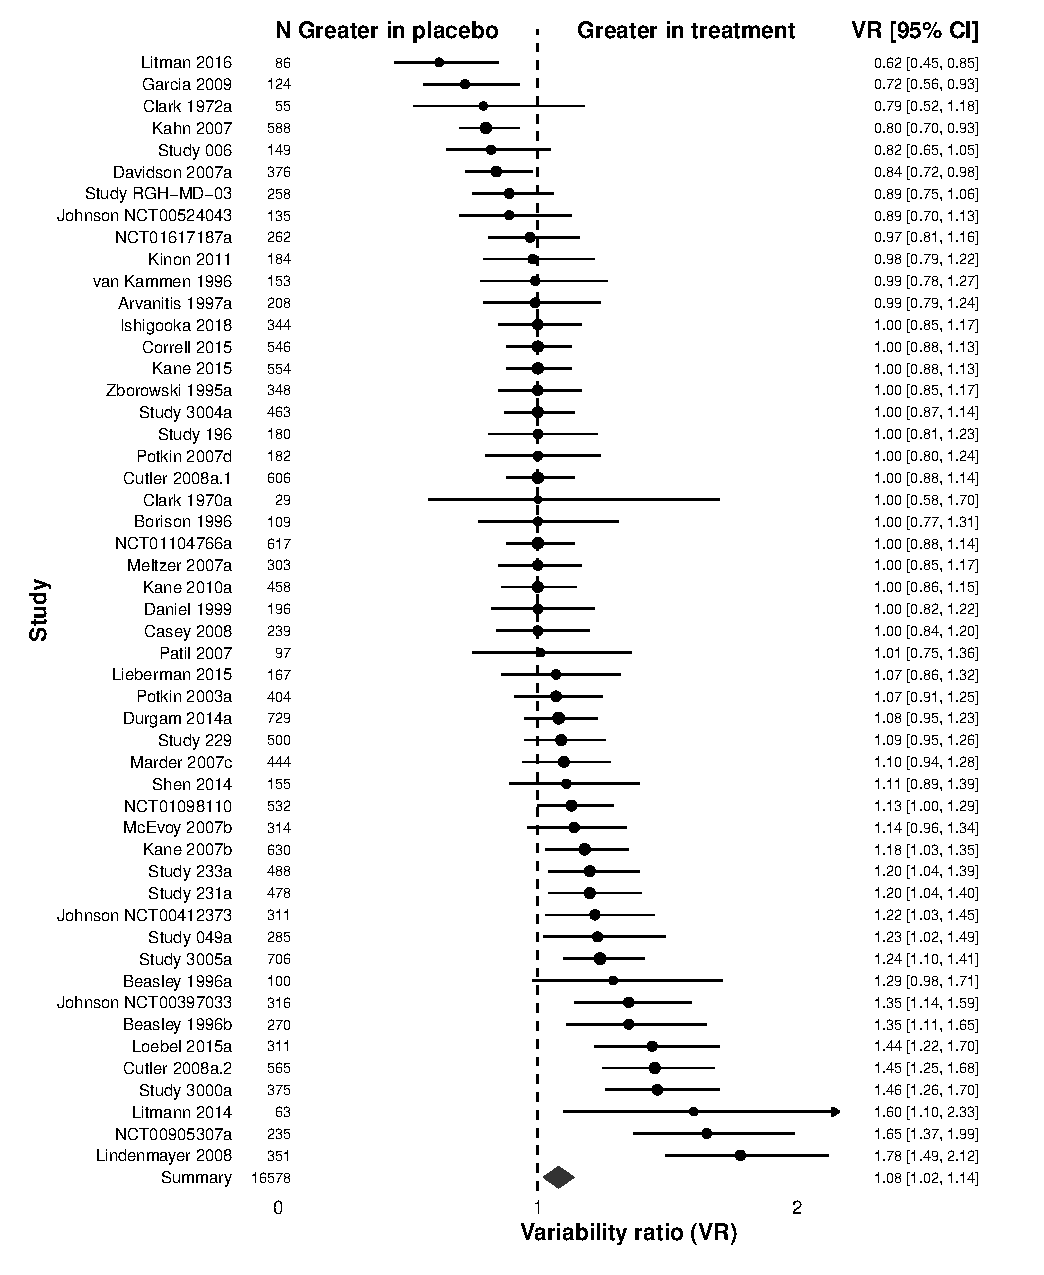
\includegraphics{../output/figures/weightsd_fig1.pdf}
\caption{\label{fig:fig1}Variability ratio for weight gain. The forest
plot shows the VR together with its 95\% confidence interval (CI) for
treatment versus placebo. All included studies\textsuperscript{41--95}
are also listed in Table S1.}
\end{figure}

\begin{figure}
\centering
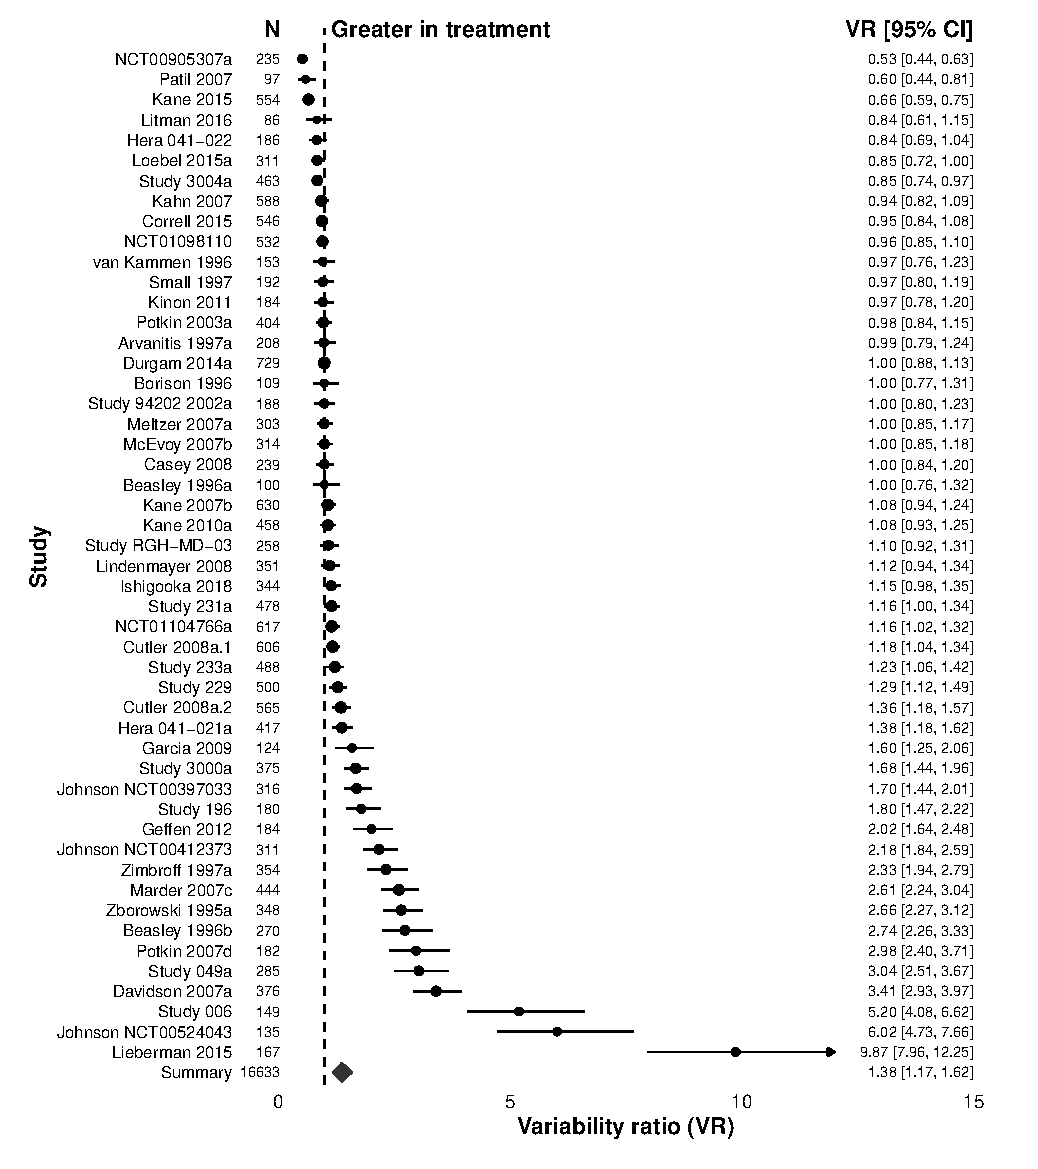
\includegraphics{../output/figures/prolactinsd_fig1.pdf}
\caption{\label{fig:fig3}Variability ratio for hyperprolactinemia. The forest
plot shows the VR together with its 95\% confidence interval (CI) for
treatment versus placebo. All included studies\textsuperscript{41,42,44--48,50--58,60,62,64,65,67--69,72,74--79,82--92,94--100}
are also listed in Table S1.}
\end{figure}

\begin{figure}
\centering
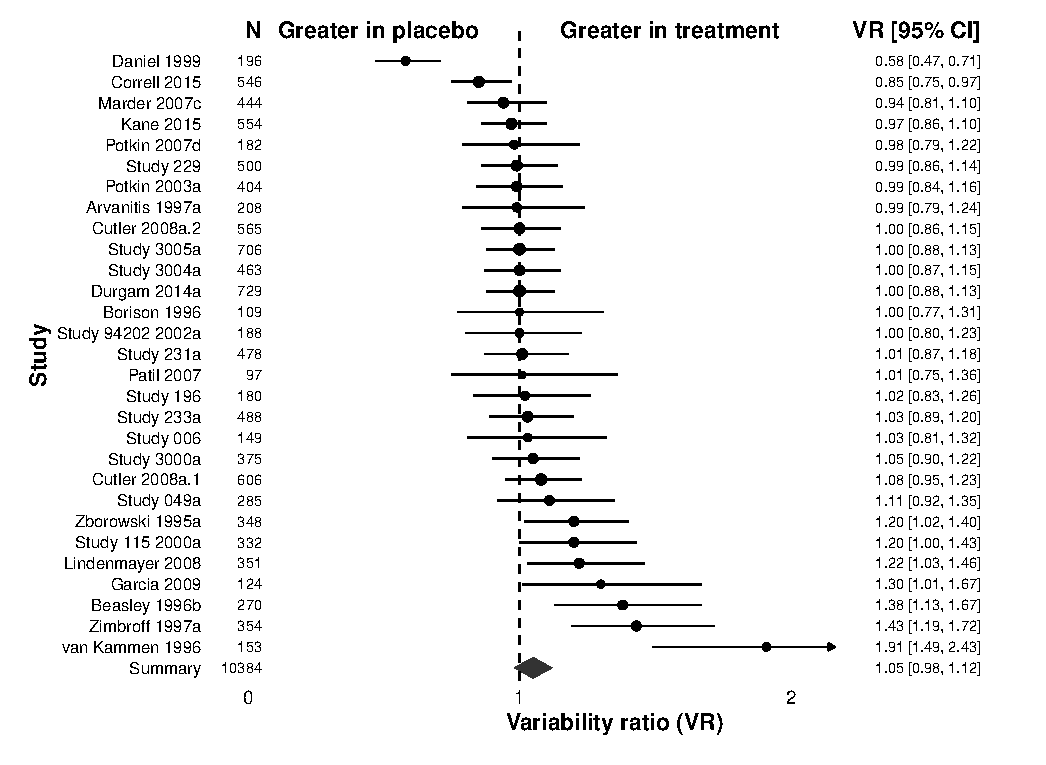
\includegraphics{../output/figures/qtcsd_fig1.pdf}
\caption{\label{fig:fig5}Variability ratio for QTc prolongation. The forest
plot shows the VR together with its 95\% confidence interval (CI) for
treatment versus placebo. All included studies\textsuperscript{42,45,51,52,54--60,62,68,70,74,76--80,85,86,88,91,95,96,100}
are also listed in Table S1.}
\end{figure}


\end{document}
